\documentclass[]{article}
\usepackage{lmodern}
\usepackage{amssymb,amsmath}
\usepackage{ifxetex,ifluatex}
\usepackage{fixltx2e} % provides \textsubscript
\ifnum 0\ifxetex 1\fi\ifluatex 1\fi=0 % if pdftex
  \usepackage[T1]{fontenc}
  \usepackage[utf8]{inputenc}
\else % if luatex or xelatex
  \ifxetex
    \usepackage{mathspec}
  \else
    \usepackage{fontspec}
  \fi
  \defaultfontfeatures{Ligatures=TeX,Scale=MatchLowercase}
\fi
% use upquote if available, for straight quotes in verbatim environments
\IfFileExists{upquote.sty}{\usepackage{upquote}}{}
% use microtype if available
\IfFileExists{microtype.sty}{%
\usepackage{microtype}
\UseMicrotypeSet[protrusion]{basicmath} % disable protrusion for tt fonts
}{}
\usepackage[margin=1in]{geometry}
\usepackage{hyperref}
\hypersetup{unicode=true,
            pdftitle={Ranking rules},
            pdfborder={0 0 0},
            breaklinks=true}
\urlstyle{same}  % don't use monospace font for urls
\usepackage{color}
\usepackage{fancyvrb}
\newcommand{\VerbBar}{|}
\newcommand{\VERB}{\Verb[commandchars=\\\{\}]}
\DefineVerbatimEnvironment{Highlighting}{Verbatim}{commandchars=\\\{\}}
% Add ',fontsize=\small' for more characters per line
\usepackage{framed}
\definecolor{shadecolor}{RGB}{248,248,248}
\newenvironment{Shaded}{\begin{snugshade}}{\end{snugshade}}
\newcommand{\AlertTok}[1]{\textcolor[rgb]{0.94,0.16,0.16}{#1}}
\newcommand{\AnnotationTok}[1]{\textcolor[rgb]{0.56,0.35,0.01}{\textbf{\textit{#1}}}}
\newcommand{\AttributeTok}[1]{\textcolor[rgb]{0.77,0.63,0.00}{#1}}
\newcommand{\BaseNTok}[1]{\textcolor[rgb]{0.00,0.00,0.81}{#1}}
\newcommand{\BuiltInTok}[1]{#1}
\newcommand{\CharTok}[1]{\textcolor[rgb]{0.31,0.60,0.02}{#1}}
\newcommand{\CommentTok}[1]{\textcolor[rgb]{0.56,0.35,0.01}{\textit{#1}}}
\newcommand{\CommentVarTok}[1]{\textcolor[rgb]{0.56,0.35,0.01}{\textbf{\textit{#1}}}}
\newcommand{\ConstantTok}[1]{\textcolor[rgb]{0.00,0.00,0.00}{#1}}
\newcommand{\ControlFlowTok}[1]{\textcolor[rgb]{0.13,0.29,0.53}{\textbf{#1}}}
\newcommand{\DataTypeTok}[1]{\textcolor[rgb]{0.13,0.29,0.53}{#1}}
\newcommand{\DecValTok}[1]{\textcolor[rgb]{0.00,0.00,0.81}{#1}}
\newcommand{\DocumentationTok}[1]{\textcolor[rgb]{0.56,0.35,0.01}{\textbf{\textit{#1}}}}
\newcommand{\ErrorTok}[1]{\textcolor[rgb]{0.64,0.00,0.00}{\textbf{#1}}}
\newcommand{\ExtensionTok}[1]{#1}
\newcommand{\FloatTok}[1]{\textcolor[rgb]{0.00,0.00,0.81}{#1}}
\newcommand{\FunctionTok}[1]{\textcolor[rgb]{0.00,0.00,0.00}{#1}}
\newcommand{\ImportTok}[1]{#1}
\newcommand{\InformationTok}[1]{\textcolor[rgb]{0.56,0.35,0.01}{\textbf{\textit{#1}}}}
\newcommand{\KeywordTok}[1]{\textcolor[rgb]{0.13,0.29,0.53}{\textbf{#1}}}
\newcommand{\NormalTok}[1]{#1}
\newcommand{\OperatorTok}[1]{\textcolor[rgb]{0.81,0.36,0.00}{\textbf{#1}}}
\newcommand{\OtherTok}[1]{\textcolor[rgb]{0.56,0.35,0.01}{#1}}
\newcommand{\PreprocessorTok}[1]{\textcolor[rgb]{0.56,0.35,0.01}{\textit{#1}}}
\newcommand{\RegionMarkerTok}[1]{#1}
\newcommand{\SpecialCharTok}[1]{\textcolor[rgb]{0.00,0.00,0.00}{#1}}
\newcommand{\SpecialStringTok}[1]{\textcolor[rgb]{0.31,0.60,0.02}{#1}}
\newcommand{\StringTok}[1]{\textcolor[rgb]{0.31,0.60,0.02}{#1}}
\newcommand{\VariableTok}[1]{\textcolor[rgb]{0.00,0.00,0.00}{#1}}
\newcommand{\VerbatimStringTok}[1]{\textcolor[rgb]{0.31,0.60,0.02}{#1}}
\newcommand{\WarningTok}[1]{\textcolor[rgb]{0.56,0.35,0.01}{\textbf{\textit{#1}}}}
\usepackage{graphicx,grffile}
\makeatletter
\def\maxwidth{\ifdim\Gin@nat@width>\linewidth\linewidth\else\Gin@nat@width\fi}
\def\maxheight{\ifdim\Gin@nat@height>\textheight\textheight\else\Gin@nat@height\fi}
\makeatother
% Scale images if necessary, so that they will not overflow the page
% margins by default, and it is still possible to overwrite the defaults
% using explicit options in \includegraphics[width, height, ...]{}
\setkeys{Gin}{width=\maxwidth,height=\maxheight,keepaspectratio}
\IfFileExists{parskip.sty}{%
\usepackage{parskip}
}{% else
\setlength{\parindent}{0pt}
\setlength{\parskip}{6pt plus 2pt minus 1pt}
}
\setlength{\emergencystretch}{3em}  % prevent overfull lines
\providecommand{\tightlist}{%
  \setlength{\itemsep}{0pt}\setlength{\parskip}{0pt}}
\setcounter{secnumdepth}{0}
% Redefines (sub)paragraphs to behave more like sections
\ifx\paragraph\undefined\else
\let\oldparagraph\paragraph
\renewcommand{\paragraph}[1]{\oldparagraph{#1}\mbox{}}
\fi
\ifx\subparagraph\undefined\else
\let\oldsubparagraph\subparagraph
\renewcommand{\subparagraph}[1]{\oldsubparagraph{#1}\mbox{}}
\fi

%%% Use protect on footnotes to avoid problems with footnotes in titles
\let\rmarkdownfootnote\footnote%
\def\footnote{\protect\rmarkdownfootnote}

%%% Change title format to be more compact
\usepackage{titling}

% Create subtitle command for use in maketitle
\providecommand{\subtitle}[1]{
  \posttitle{
    \begin{center}\large#1\end{center}
    }
}

\setlength{\droptitle}{-2em}

  \title{Ranking rules}
    \pretitle{\vspace{\droptitle}\centering\huge}
  \posttitle{\par}
    \author{}
    \preauthor{}\postauthor{}
    \date{}
    \predate{}\postdate{}
  

\begin{document}
\maketitle

Dados los siguientes puntos:

\includegraphics{Example_files/figure-latex/unnamed-chunk-3-1.pdf}

Calculamos los puntos más cercanos a X utilizando las distancias:

\begin{itemize}
\tightlist
\item
  Manhattan
\item
  Euclidea
\item
  Chebyshev
\end{itemize}

\textbf{Manhattan}

\begin{Shaded}
\begin{Highlighting}[]
\NormalTok{manhattan <-}\StringTok{ }\KeywordTok{as.matrix}\NormalTok{(}\KeywordTok{dist}\NormalTok{(points[,}\OperatorTok{-}\KeywordTok{c}\NormalTok{(}\DecValTok{3}\NormalTok{,}\DecValTok{4}\NormalTok{)], }\DataTypeTok{method =} \StringTok{"manhattan"}\NormalTok{))[}\DecValTok{1}\NormalTok{,}\OperatorTok{-}\DecValTok{1}\NormalTok{]}
\KeywordTok{names}\NormalTok{(manhattan) <-}\StringTok{ }\NormalTok{LETTERS[}\DecValTok{1}\OperatorTok{:}\KeywordTok{length}\NormalTok{(manhattan)]}
\NormalTok{manhattan}
\end{Highlighting}
\end{Shaded}

\begin{verbatim}
##        A        B        C        D        E        F 
## 3.000000 3.000000 3.000000 3.000000 4.000000 3.645751
\end{verbatim}

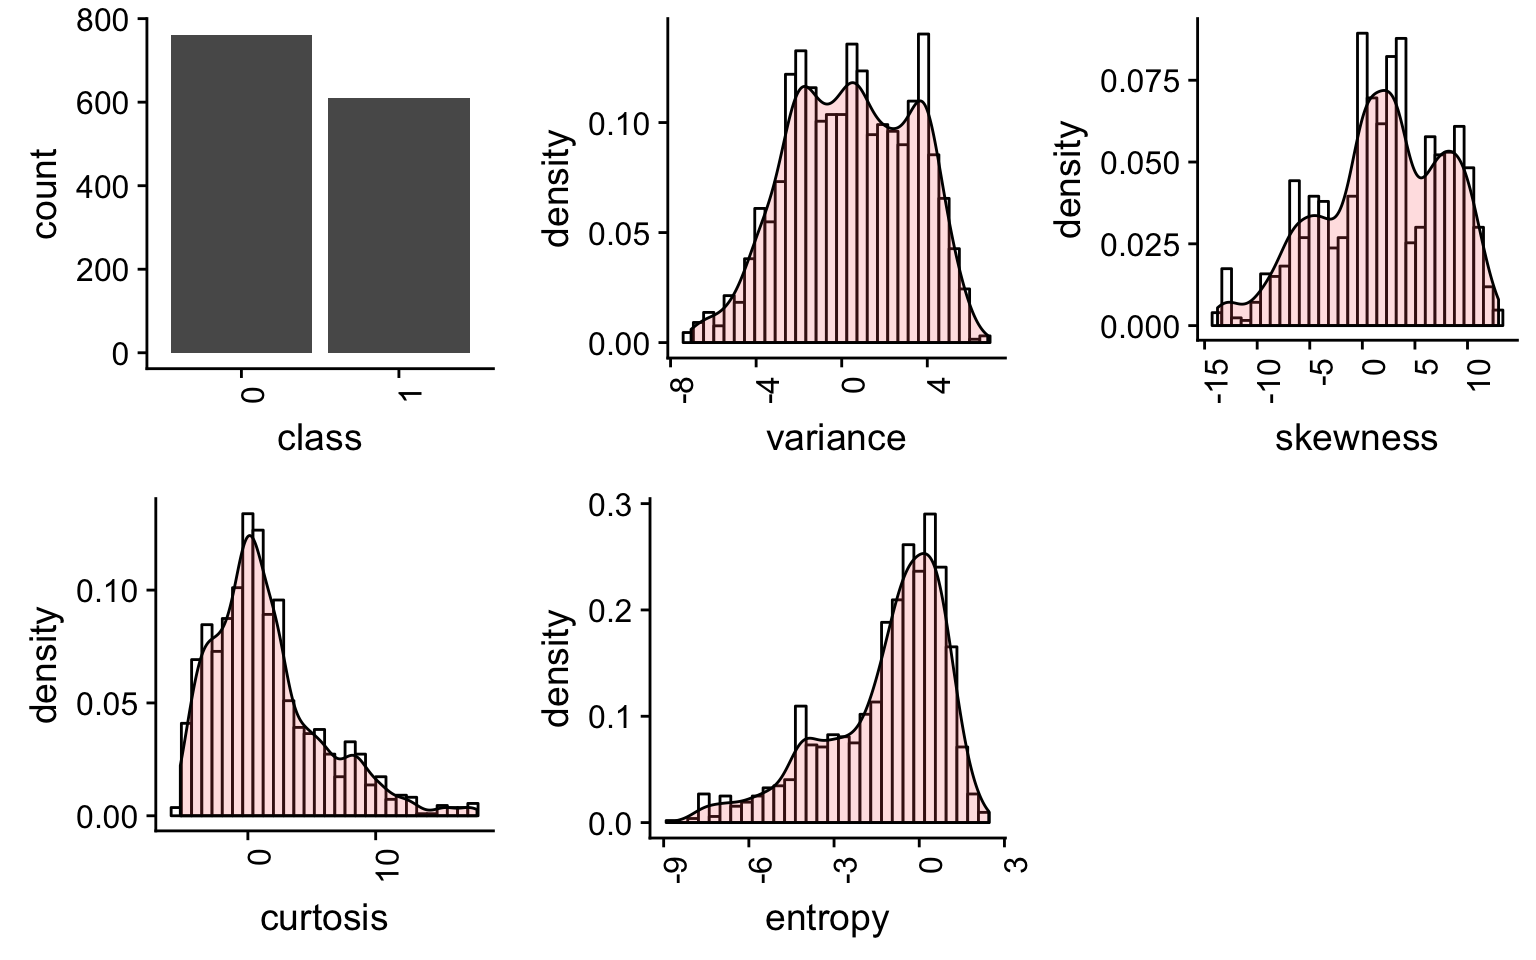
\includegraphics{Example_files/figure-latex/unnamed-chunk-5-1.pdf}

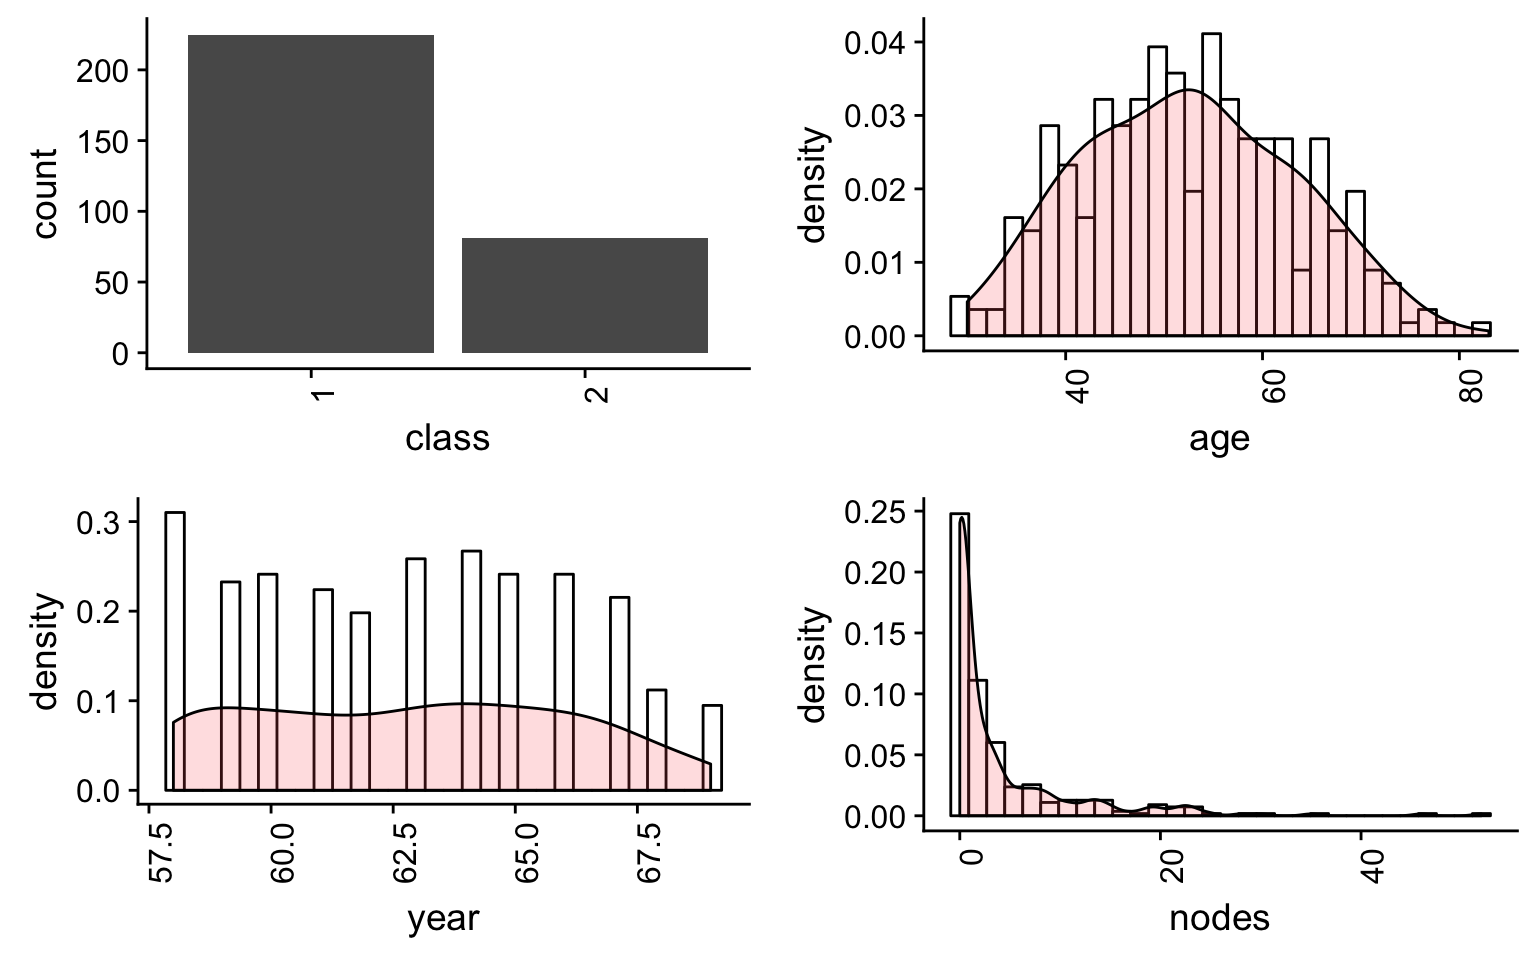
\includegraphics{Example_files/figure-latex/unnamed-chunk-6-1.pdf}

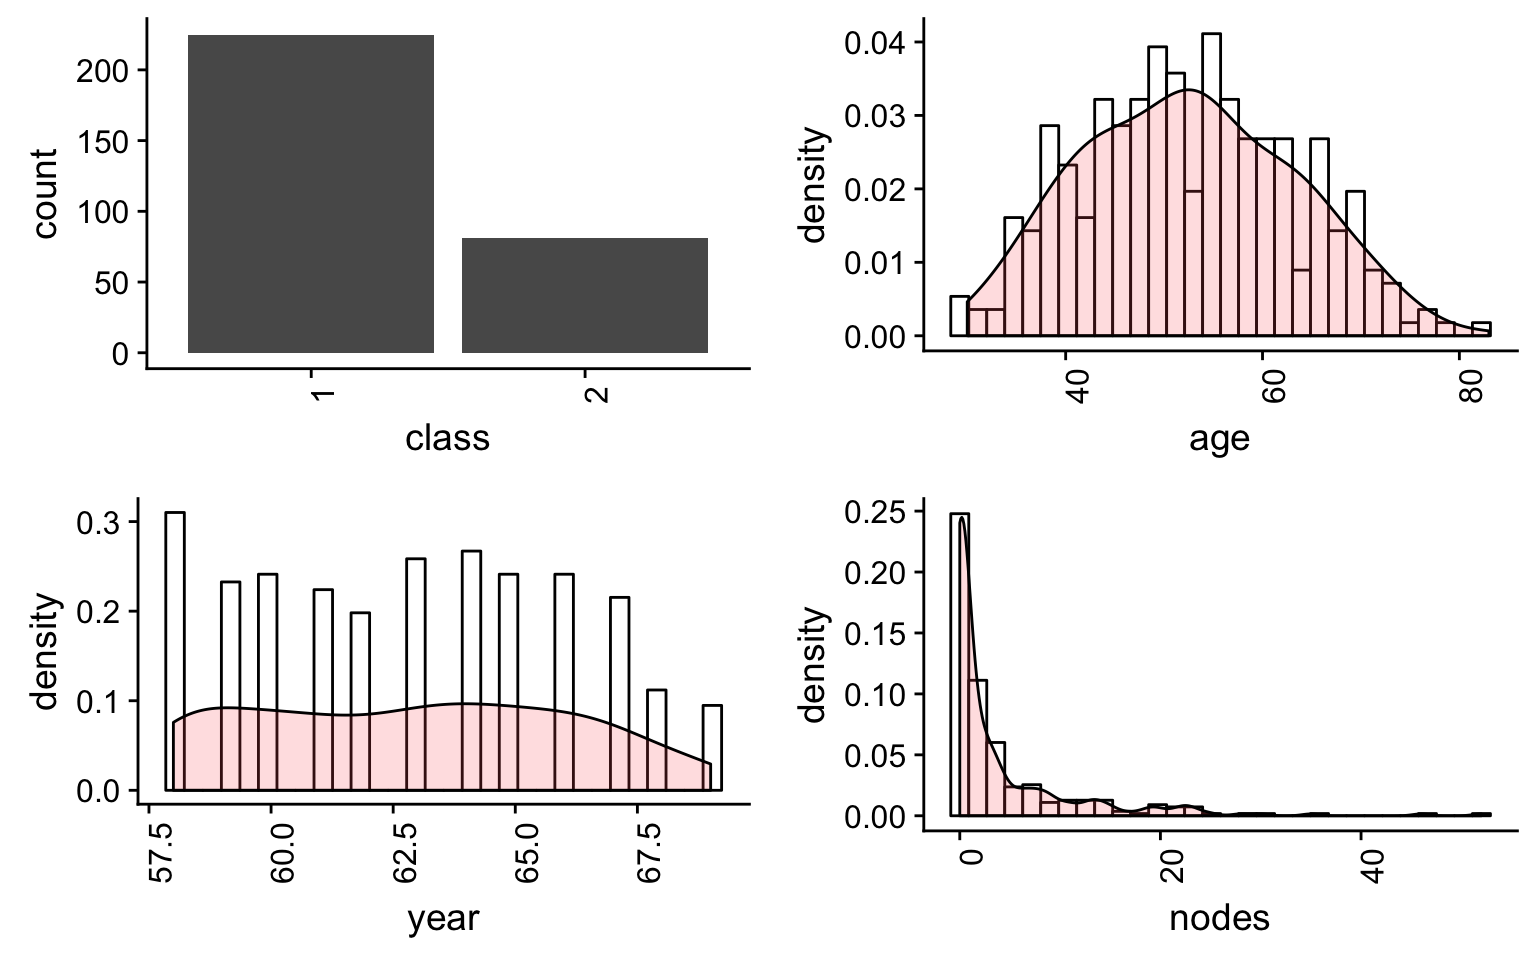
\includegraphics{Example_files/figure-latex/unnamed-chunk-7-1.pdf}

\textbf{Euclidea}

\begin{Shaded}
\begin{Highlighting}[]
\NormalTok{euclidean <-}\StringTok{ }\KeywordTok{as.matrix}\NormalTok{(}\KeywordTok{dist}\NormalTok{(points[,}\OperatorTok{-}\KeywordTok{c}\NormalTok{(}\DecValTok{3}\NormalTok{,}\DecValTok{4}\NormalTok{)], }\DataTypeTok{method =} \StringTok{"euclidean"}\NormalTok{))[}\DecValTok{1}\NormalTok{,}\OperatorTok{-}\DecValTok{1}\NormalTok{]}
\KeywordTok{names}\NormalTok{(euclidean) <-}\StringTok{ }\NormalTok{LETTERS[}\DecValTok{1}\OperatorTok{:}\KeywordTok{length}\NormalTok{(euclidean)]}
\NormalTok{euclidean}
\end{Highlighting}
\end{Shaded}

\begin{verbatim}
##        A        B        C        D        E        F 
## 3.000000 2.236068 2.236068 3.000000 2.828427 2.828427
\end{verbatim}

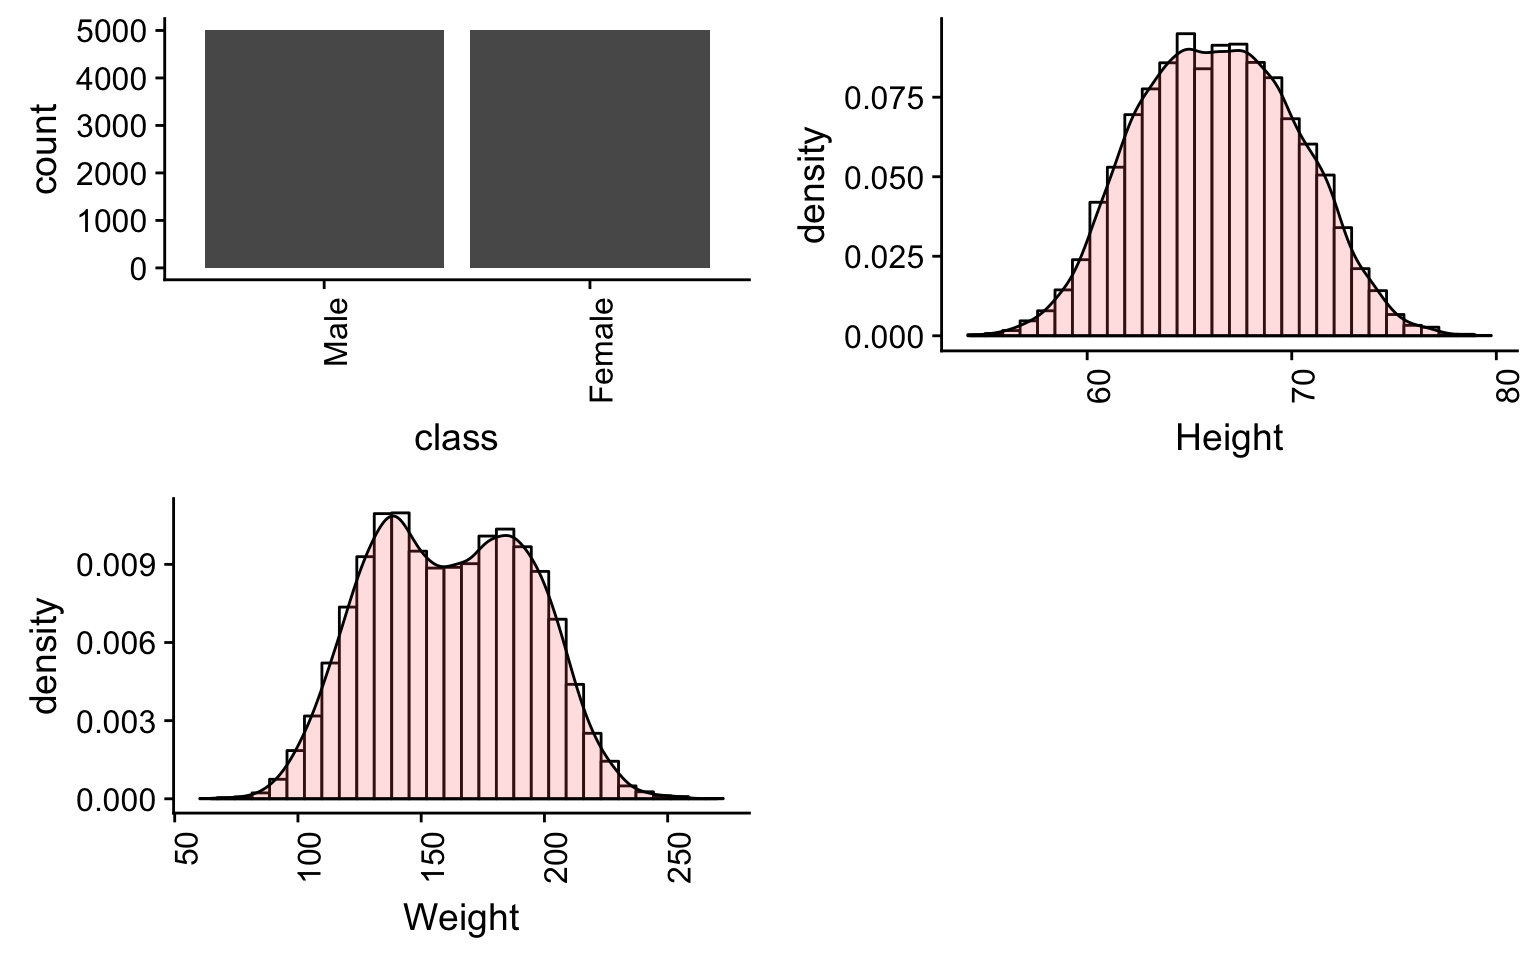
\includegraphics{Example_files/figure-latex/unnamed-chunk-9-1.pdf}

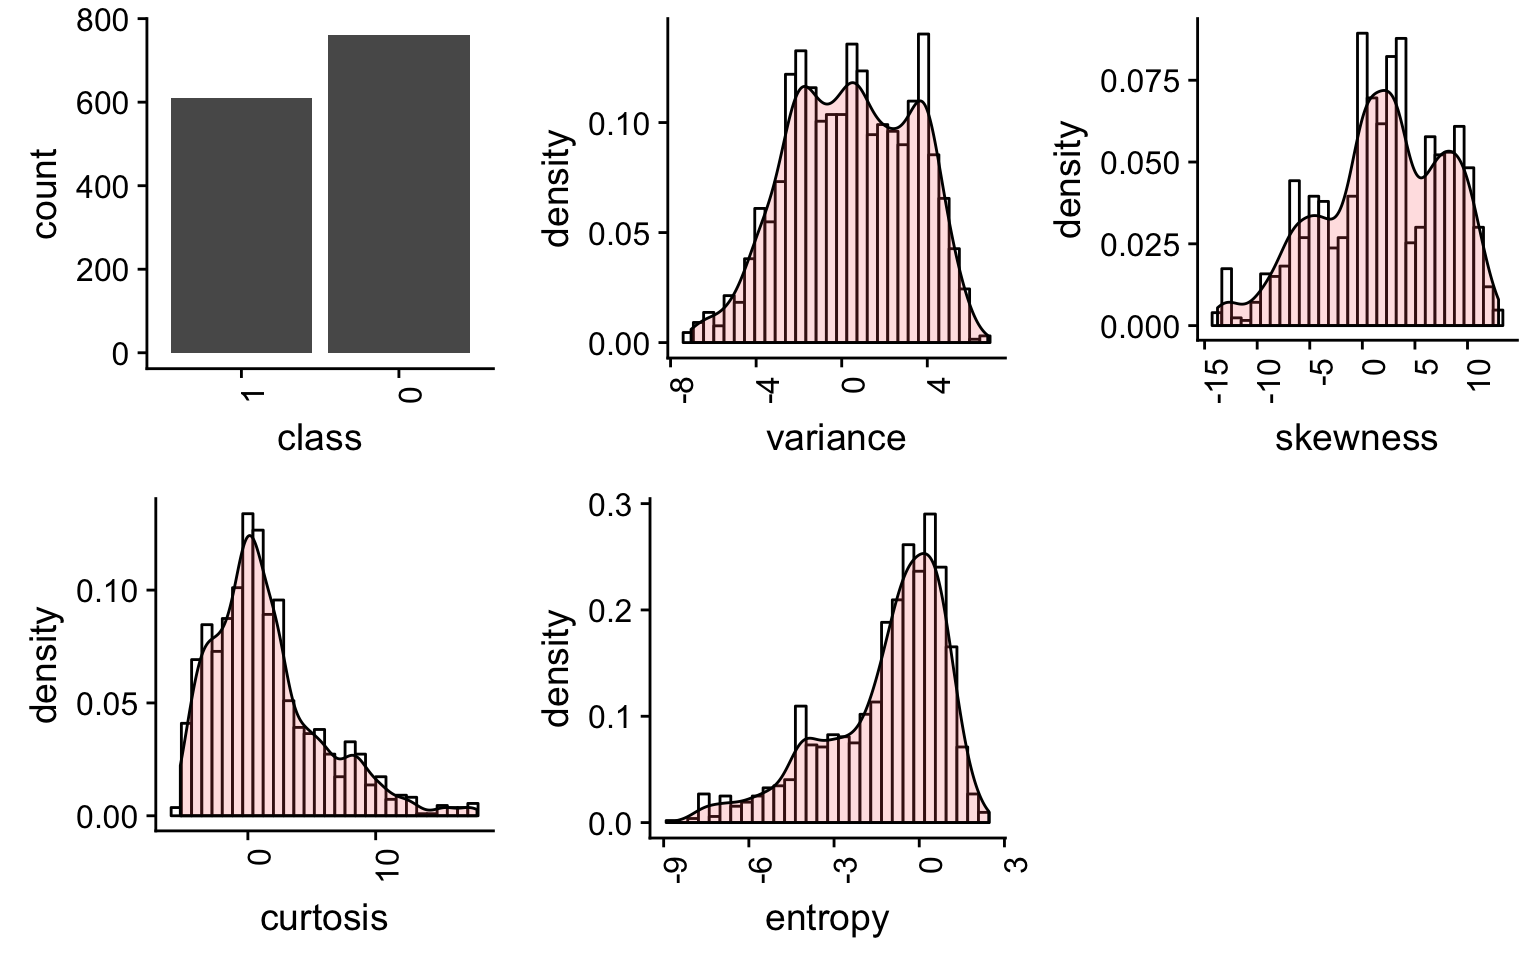
\includegraphics{Example_files/figure-latex/unnamed-chunk-10-1.pdf}

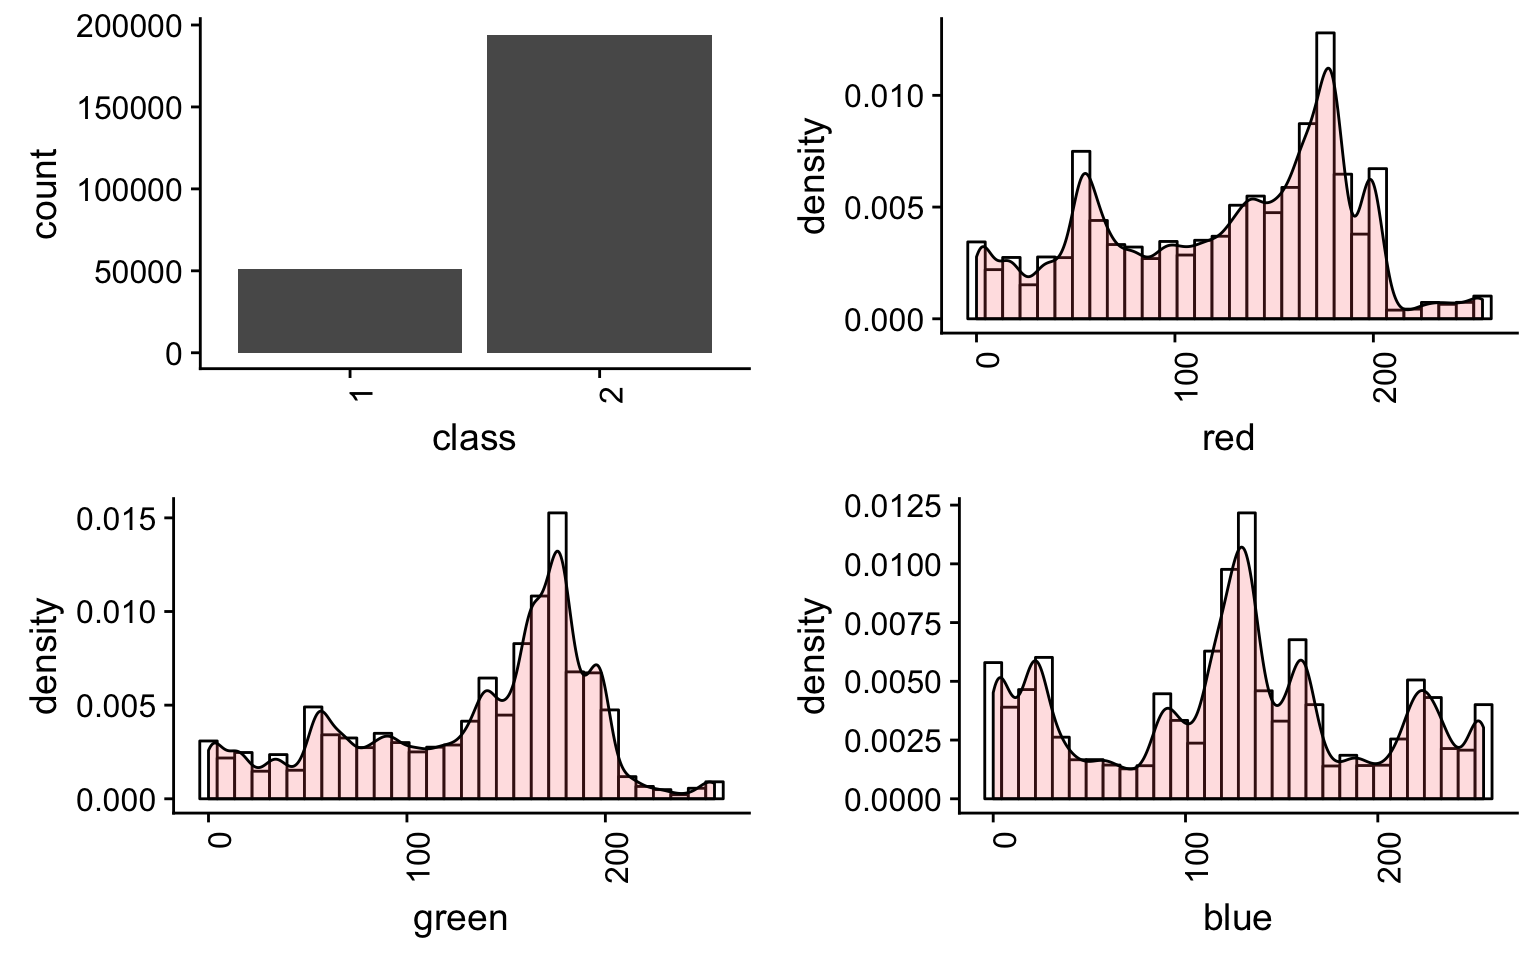
\includegraphics{Example_files/figure-latex/unnamed-chunk-11-1.pdf}

\textbf{Chebyshev}

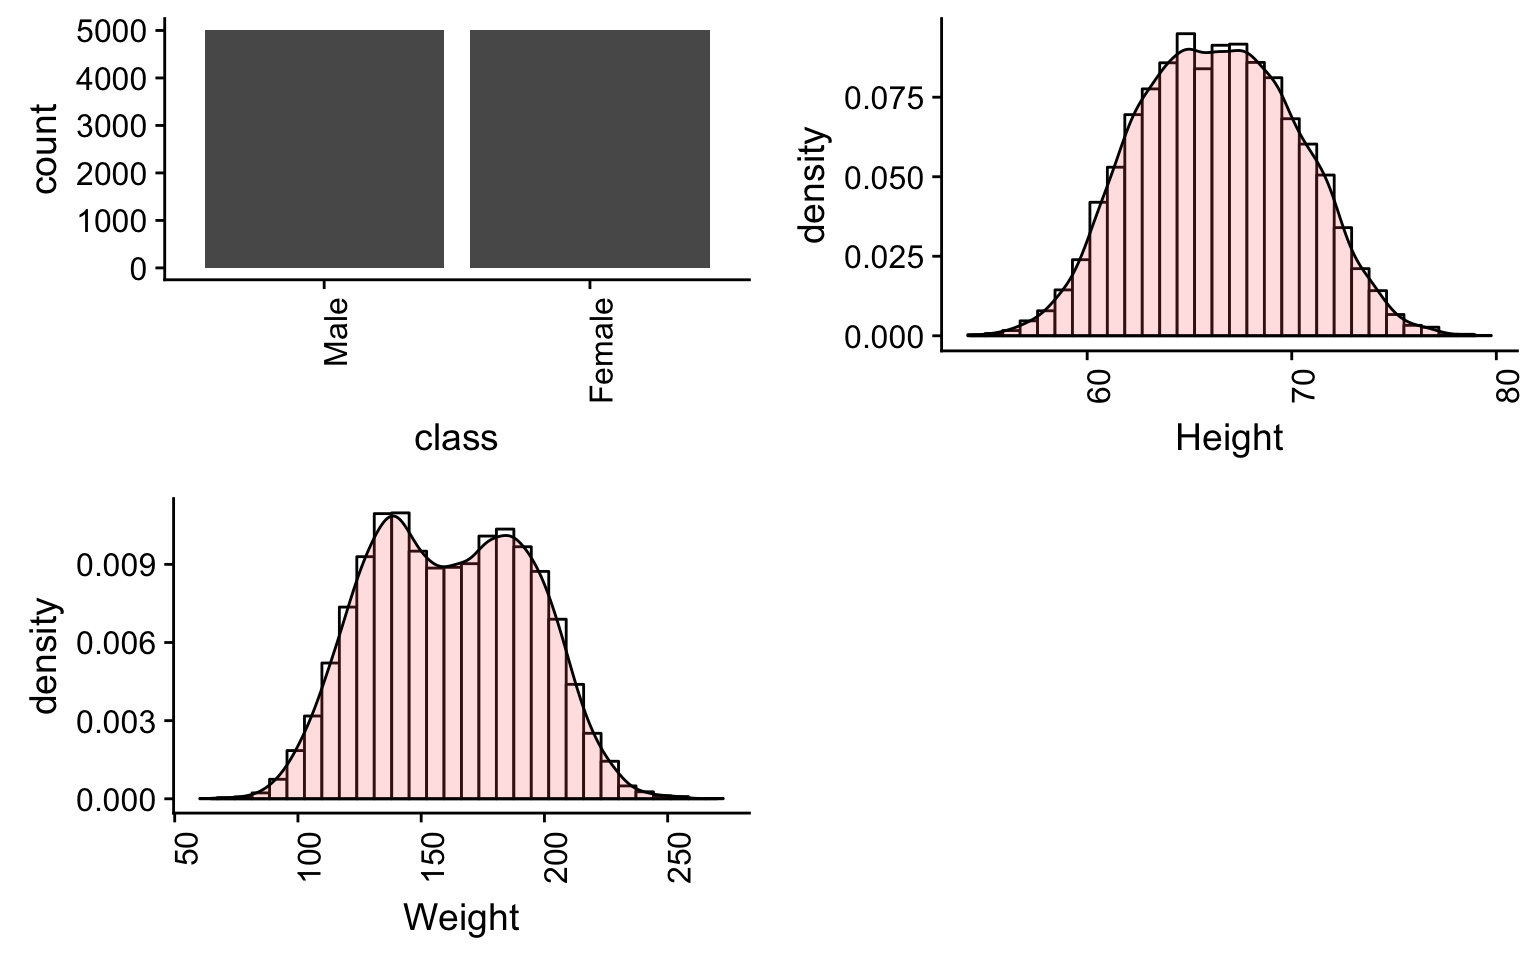
\includegraphics{Example_files/figure-latex/unnamed-chunk-12-1.pdf}

\begin{verbatim}
## Warning: Duplicated aesthetics after name standardisation: size
\end{verbatim}

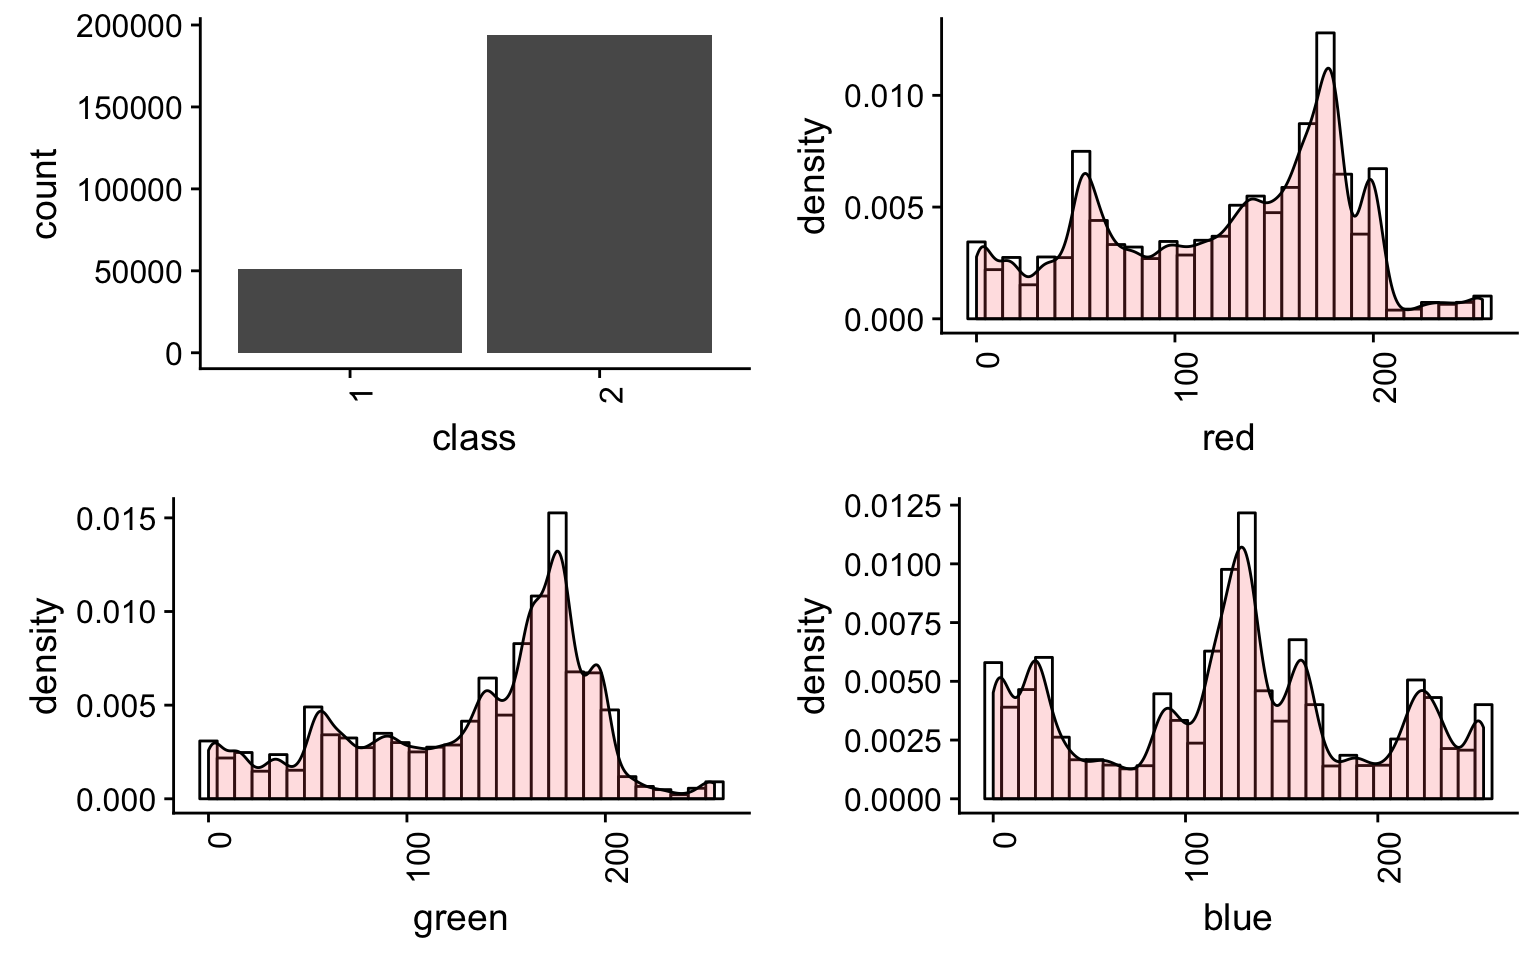
\includegraphics{Example_files/figure-latex/unnamed-chunk-13-1.pdf}

\begin{verbatim}
## Warning: Duplicated aesthetics after name standardisation: size
\end{verbatim}

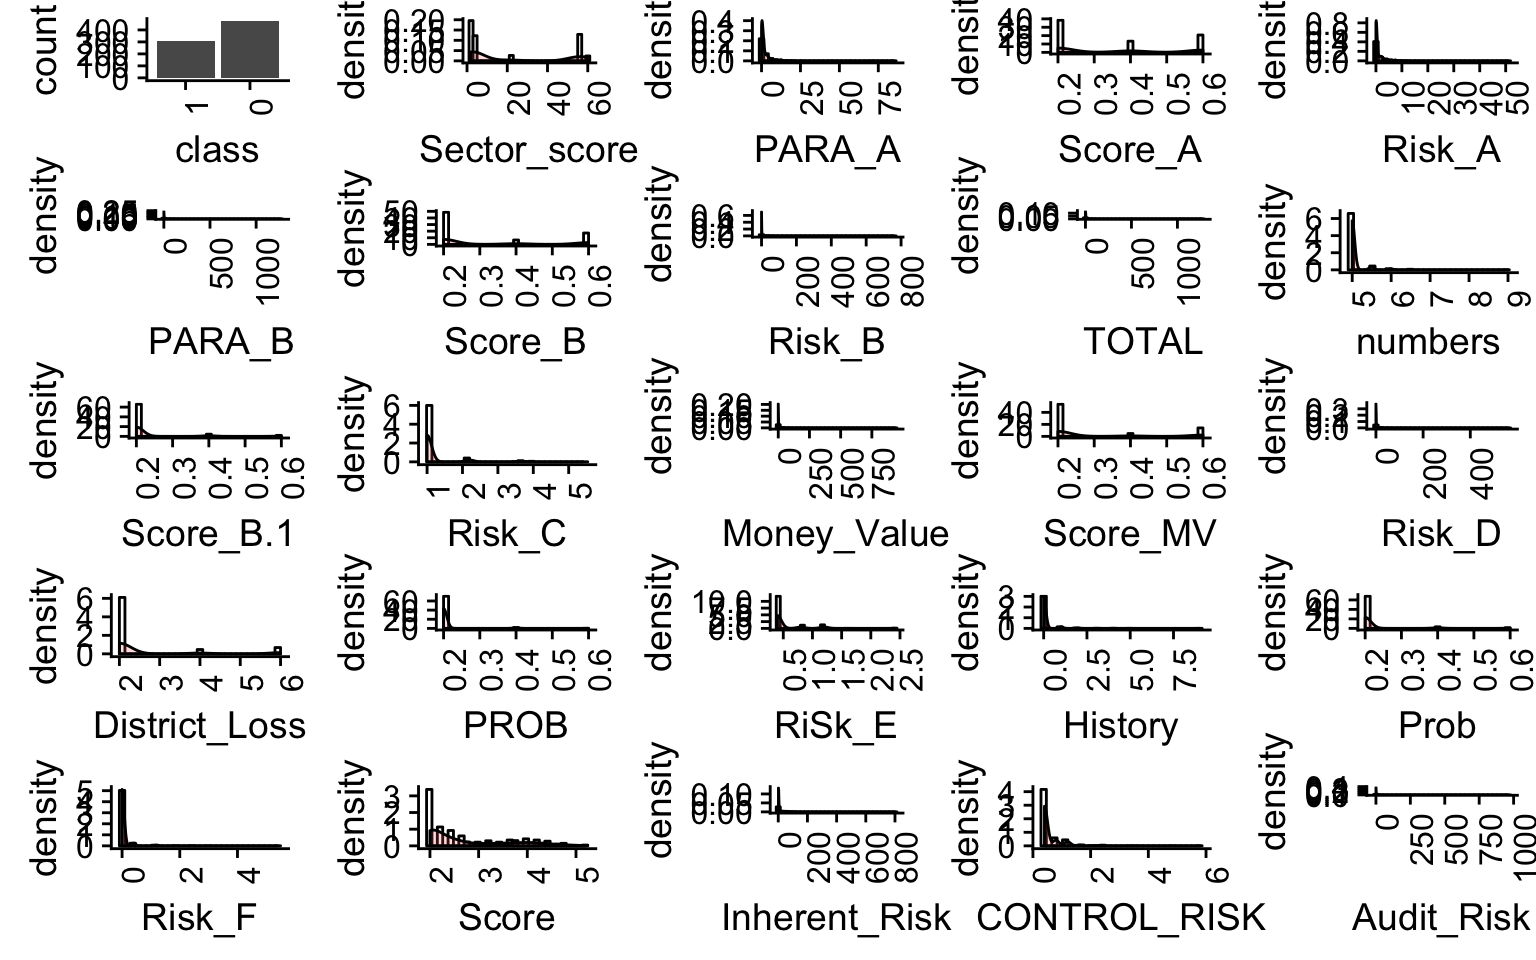
\includegraphics{Example_files/figure-latex/unnamed-chunk-14-1.pdf}

\hypertarget{aplicando-reglas}{%
\subsection{Aplicando reglas}\label{aplicando-reglas}}

Apply plurality:

\[
\begin{center}
\begin{tabular}{ c c c c c c}
 B & C & D & E & F & G
 \frac{1}{4} & \frac{1}{4} & \frac{1}{4} & \frac{1}{4} & 0 & 0 \\ 
 0 & \frac{1}{2} & \frac{1}{2} & 0 & 0 & 0 \\  
 0 & \frac{1}{4} & \frac{1}{4} & 0 & \frac{1}{4} & \frac{1}{4} \\ 
\end{tabular}
\end{center}
\]

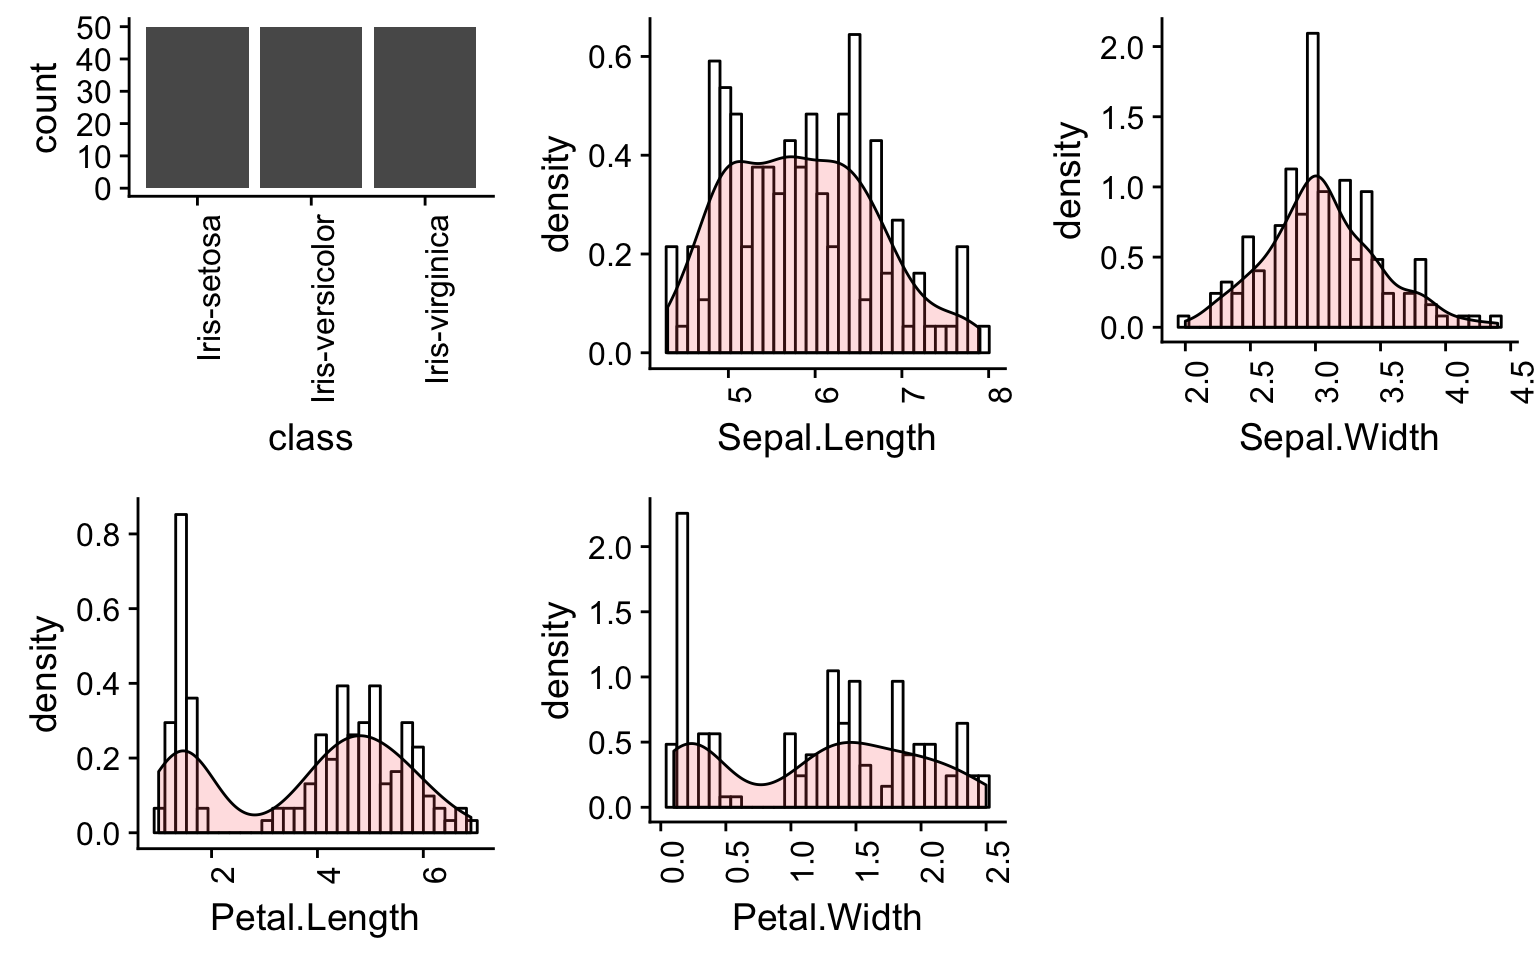
\includegraphics{Example_files/figure-latex/unnamed-chunk-15-1.pdf}

\begin{Shaded}
\begin{Highlighting}[]
\NormalTok{chebyshev <-}\StringTok{ }\KeywordTok{as.matrix}\NormalTok{(}\KeywordTok{dist}\NormalTok{(points[,}\OperatorTok{-}\DecValTok{3}\NormalTok{], }\DataTypeTok{method =} \StringTok{"maximum"}\NormalTok{))[}\DecValTok{1}\NormalTok{,}\OperatorTok{-}\DecValTok{1}\NormalTok{]}
\end{Highlighting}
\end{Shaded}

\begin{verbatim}
## Warning in dist(points[, -3], method = "maximum"): NAs introduced by
## coercion
\end{verbatim}

\begin{Shaded}
\begin{Highlighting}[]
\KeywordTok{names}\NormalTok{(chebyshev) <-}\StringTok{ }\NormalTok{LETTERS[}\DecValTok{1}\OperatorTok{:}\KeywordTok{length}\NormalTok{(chebyshev)]}
\NormalTok{chebyshev}
\end{Highlighting}
\end{Shaded}

\begin{verbatim}
##        A        B        C        D        E        F 
## 3.000000 2.000000 2.000000 3.000000 2.000000 2.645751
\end{verbatim}

\begin{Shaded}
\begin{Highlighting}[]
\NormalTok{rankings <-}\StringTok{ }\KeywordTok{bind_rows}\NormalTok{(manhattan, }
\NormalTok{          euclidean,}
\NormalTok{          chebyshev)}
\NormalTok{rankings <-}\StringTok{ }\KeywordTok{t}\NormalTok{(}\KeywordTok{apply}\NormalTok{(rankings, }\DecValTok{1}\NormalTok{, ranking))}
\KeywordTok{rownames}\NormalTok{(rankings) <-}\StringTok{ }\KeywordTok{c}\NormalTok{(}\StringTok{"manhattan"}\NormalTok{, }\StringTok{"euclidean"}\NormalTok{, }\StringTok{"chebyshev"}\NormalTok{)}
\NormalTok{rankings <-}\StringTok{ }\KeywordTok{profile_of_rankings}\NormalTok{(rankings)}
\end{Highlighting}
\end{Shaded}

\begin{Shaded}
\begin{Highlighting}[]
\KeywordTok{plurality}\NormalTok{(rankings)}
\end{Highlighting}
\end{Shaded}

\begin{verbatim}
## B ~ C > E > A ~ D > F
\end{verbatim}

\begin{verbatim}
## B ~ C > E > A ~ D > F
\end{verbatim}

\begin{Shaded}
\begin{Highlighting}[]
\KeywordTok{borda_count}\NormalTok{(rankings)}
\end{Highlighting}
\end{Shaded}

\begin{verbatim}
## B ~ C > E > F > A ~ D
\end{verbatim}

\begin{verbatim}
## B ~ C > E > F > A ~ D
\end{verbatim}

\begin{Shaded}
\begin{Highlighting}[]
\KeywordTok{two}\NormalTok{(rankings)}
\end{Highlighting}
\end{Shaded}

\begin{verbatim}
## B ~ C > E > A ~ D > F
\end{verbatim}

\begin{verbatim}
## B ~ C > E > A ~ D > F
\end{verbatim}

\begin{Shaded}
\begin{Highlighting}[]
\KeywordTok{three}\NormalTok{(rankings)}
\end{Highlighting}
\end{Shaded}

\begin{verbatim}
## B ~ C > E > A ~ D > F
\end{verbatim}

\begin{verbatim}
## B ~ C > E > A ~ D > F
\end{verbatim}

\begin{Shaded}
\begin{Highlighting}[]
\KeywordTok{five}\NormalTok{(rankings)}
\end{Highlighting}
\end{Shaded}

\begin{verbatim}
## B ~ C ~ F > A ~ D ~ E
\end{verbatim}

\begin{verbatim}
## B ~ C ~ F > A ~ D ~ E
\end{verbatim}

\begin{Shaded}
\begin{Highlighting}[]
\KeywordTok{seven}\NormalTok{(rankings)}
\end{Highlighting}
\end{Shaded}

\begin{verbatim}
## A ~ B ~ C ~ D ~ E ~ F
\end{verbatim}

\begin{verbatim}
## A ~ B ~ C ~ D ~ E ~ F
\end{verbatim}

\begin{Shaded}
\begin{Highlighting}[]
\KeywordTok{ggplot}\NormalTok{() }\OperatorTok{+}
\StringTok{  }\CommentTok{# Manhattan}
\StringTok{  }\KeywordTok{geom_polygon}\NormalTok{(}\KeywordTok{aes}\NormalTok{(}\DataTypeTok{x=}\KeywordTok{c}\NormalTok{(}\OperatorTok{-}\DecValTok{3}\NormalTok{,}\DecValTok{0}\NormalTok{,}\DecValTok{3}\NormalTok{,}\DecValTok{0}\NormalTok{), }\DataTypeTok{y =} \KeywordTok{c}\NormalTok{(}\DecValTok{0}\NormalTok{,}\DecValTok{3}\NormalTok{,}\DecValTok{0}\NormalTok{,}\OperatorTok{-}\DecValTok{3}\NormalTok{), }\DataTypeTok{linetype =}\NormalTok{ b), }\DataTypeTok{fill =} \StringTok{"black"}\NormalTok{, }\DataTypeTok{color=}\NormalTok{color_manhattan, }\DataTypeTok{alpha=}\DecValTok{0}\NormalTok{, }\DataTypeTok{linetype =} \StringTok{"twodash"}\NormalTok{) }\OperatorTok{+}
\StringTok{  }\KeywordTok{geom_polygon}\NormalTok{(}\KeywordTok{aes}\NormalTok{(}\DataTypeTok{x=}\KeywordTok{c}\NormalTok{(}\OperatorTok{-}\DecValTok{4}\NormalTok{,}\DecValTok{0}\NormalTok{,}\DecValTok{4}\NormalTok{,}\DecValTok{0}\NormalTok{), }\DataTypeTok{y =} \KeywordTok{c}\NormalTok{(}\DecValTok{0}\NormalTok{,}\DecValTok{4}\NormalTok{,}\DecValTok{0}\NormalTok{,}\OperatorTok{-}\DecValTok{4}\NormalTok{)), }\DataTypeTok{fill =} \StringTok{"black"}\NormalTok{, }\DataTypeTok{color=}\NormalTok{color_manhattan, }\DataTypeTok{alpha=}\DecValTok{0}\NormalTok{, }\DataTypeTok{linetype =} \StringTok{"twodash"}\NormalTok{) }\OperatorTok{+}
\StringTok{  }\KeywordTok{geom_polygon}\NormalTok{(}\KeywordTok{aes}\NormalTok{(}\DataTypeTok{x=}\KeywordTok{c}\NormalTok{(}\OperatorTok{-}\NormalTok{(}\KeywordTok{sqrt}\NormalTok{(}\DecValTok{7}\NormalTok{)}\OperatorTok{+}\DecValTok{1}\NormalTok{),}\DecValTok{0}\NormalTok{,(}\KeywordTok{sqrt}\NormalTok{(}\DecValTok{7}\NormalTok{)}\OperatorTok{+}\DecValTok{1}\NormalTok{),}\DecValTok{0}\NormalTok{), }\DataTypeTok{y =} \KeywordTok{c}\NormalTok{(}\DecValTok{0}\NormalTok{,(}\KeywordTok{sqrt}\NormalTok{(}\DecValTok{7}\NormalTok{)}\OperatorTok{+}\DecValTok{1}\NormalTok{),}\DecValTok{0}\NormalTok{,}\OperatorTok{-}\NormalTok{(}\KeywordTok{sqrt}\NormalTok{(}\DecValTok{7}\NormalTok{)}\OperatorTok{+}\DecValTok{1}\NormalTok{))), }\DataTypeTok{fill =} \StringTok{"black"}\NormalTok{, }\DataTypeTok{color=}\NormalTok{color_manhattan, }\DataTypeTok{alpha=}\DecValTok{0}\NormalTok{, }\DataTypeTok{linetype =} \StringTok{"twodash"}\NormalTok{) }\OperatorTok{+}
\StringTok{ }\CommentTok{# Euclidean}
\StringTok{  }\KeywordTok{geom_circle}\NormalTok{(}\KeywordTok{aes}\NormalTok{(}\DataTypeTok{x0 =} \DecValTok{0}\NormalTok{, }\DataTypeTok{y0 =} \DecValTok{0}\NormalTok{, }\DataTypeTok{r =} \KeywordTok{sqrt}\NormalTok{(}\DecValTok{5}\NormalTok{)),  }\DataTypeTok{color=}\NormalTok{color_euclidean, }\DataTypeTok{linetype =} \StringTok{"dotted"}\NormalTok{) }\OperatorTok{+}
\StringTok{  }\KeywordTok{geom_circle}\NormalTok{(}\KeywordTok{aes}\NormalTok{(}\DataTypeTok{x0 =} \DecValTok{0}\NormalTok{, }\DataTypeTok{y0 =} \DecValTok{0}\NormalTok{, }\DataTypeTok{r =} \KeywordTok{sqrt}\NormalTok{(}\DecValTok{8}\NormalTok{)),  }\DataTypeTok{color=}\NormalTok{color_euclidean, }\DataTypeTok{linetype =} \StringTok{"dotted"}\NormalTok{) }\OperatorTok{+}
\StringTok{  }\KeywordTok{geom_circle}\NormalTok{(}\KeywordTok{aes}\NormalTok{(}\DataTypeTok{x0 =} \DecValTok{0}\NormalTok{, }\DataTypeTok{y0 =} \DecValTok{0}\NormalTok{, }\DataTypeTok{r =} \DecValTok{3}\NormalTok{),  }\DataTypeTok{color=}\NormalTok{color_euclidean, }\DataTypeTok{linetype =} \StringTok{"dotted"}\NormalTok{) }\OperatorTok{+}
\StringTok{  }\CommentTok{# Chebyshev}
\StringTok{  }\KeywordTok{geom_rect}\NormalTok{(}\KeywordTok{aes}\NormalTok{(}\DataTypeTok{xmin=}\OperatorTok{-}\DecValTok{2}\NormalTok{, }\DataTypeTok{ymin=}\OperatorTok{-}\DecValTok{2}\NormalTok{, }\DataTypeTok{xmax=}\DecValTok{2}\NormalTok{, }\DataTypeTok{ymax=}\DecValTok{2}\NormalTok{), }\DataTypeTok{fill =} \StringTok{"black"}\NormalTok{, }\DataTypeTok{color=}\NormalTok{color_chebyshev, }\DataTypeTok{alpha=}\DecValTok{0}\NormalTok{, }\DataTypeTok{linetype =} \StringTok{"longdash"}\NormalTok{) }\OperatorTok{+}
\StringTok{  }\KeywordTok{geom_rect}\NormalTok{(}\KeywordTok{aes}\NormalTok{(}\DataTypeTok{xmin=}\OperatorTok{-}\DecValTok{3}\NormalTok{, }\DataTypeTok{ymin=}\OperatorTok{-}\DecValTok{3}\NormalTok{, }\DataTypeTok{xmax=}\DecValTok{3}\NormalTok{, }\DataTypeTok{ymax=}\DecValTok{3}\NormalTok{), }\DataTypeTok{fill =} \StringTok{"black"}\NormalTok{, }\DataTypeTok{color=}\NormalTok{color_chebyshev, }\DataTypeTok{alpha=}\DecValTok{0}\NormalTok{, }\DataTypeTok{linetype =} \StringTok{"longdash"}\NormalTok{) }\OperatorTok{+}
\StringTok{  }\KeywordTok{geom_rect}\NormalTok{(}\KeywordTok{aes}\NormalTok{(}\DataTypeTok{xmin=}\OperatorTok{-}\NormalTok{(}\KeywordTok{sqrt}\NormalTok{(}\DecValTok{7}\NormalTok{)), }\DataTypeTok{ymin=}\OperatorTok{-}\NormalTok{(}\KeywordTok{sqrt}\NormalTok{(}\DecValTok{7}\NormalTok{)), }\DataTypeTok{xmax=}\NormalTok{(}\KeywordTok{sqrt}\NormalTok{(}\DecValTok{7}\NormalTok{)), }\DataTypeTok{ymax=}\NormalTok{(}\KeywordTok{sqrt}\NormalTok{(}\DecValTok{7}\NormalTok{))), }\DataTypeTok{fill =} \StringTok{"black"}\NormalTok{, }\DataTypeTok{color=}\NormalTok{color_chebyshev, }\DataTypeTok{alpha=}\DecValTok{0}\NormalTok{, }\DataTypeTok{linetype =} \StringTok{"longdash"}\NormalTok{) }\OperatorTok{+}
\StringTok{  }\CommentTok{# Plot}
\StringTok{  }\KeywordTok{geom_point}\NormalTok{(}\KeywordTok{aes}\NormalTok{(x, y, }\DataTypeTok{shape =}\NormalTok{ class, }\DataTypeTok{color =}\NormalTok{ class), }\DataTypeTok{data =}\NormalTok{ points, }\DataTypeTok{size =} \DecValTok{5}\NormalTok{) }\OperatorTok{+}
\StringTok{  }\KeywordTok{geom_text}\NormalTok{(}\KeywordTok{aes}\NormalTok{(x, y, }\DataTypeTok{label =}\NormalTok{ name), }\DataTypeTok{data =}\NormalTok{ points, }\DataTypeTok{color =} \StringTok{"white"}\NormalTok{, }\DataTypeTok{fontface =} \StringTok{"bold"}\NormalTok{, }\DataTypeTok{size =} \DecValTok{3}\NormalTok{) }\OperatorTok{+}
\StringTok{  }
\StringTok{   }\KeywordTok{scale_x_continuous}\NormalTok{(}\DataTypeTok{limits =} \KeywordTok{c}\NormalTok{(}\OperatorTok{-}\DecValTok{4}\NormalTok{, }\DecValTok{4}\NormalTok{), }\DataTypeTok{breaks =} \DecValTok{-4}\OperatorTok{:}\DecValTok{4}\NormalTok{) }\OperatorTok{+}
\StringTok{  }\KeywordTok{scale_y_continuous}\NormalTok{(}\DataTypeTok{limits =} \KeywordTok{c}\NormalTok{(}\OperatorTok{-}\DecValTok{4}\NormalTok{, }\DecValTok{4}\NormalTok{), }\DataTypeTok{breaks =} \DecValTok{-4}\OperatorTok{:}\DecValTok{4}\NormalTok{) }\OperatorTok{+}
\StringTok{  }\KeywordTok{scale_colour_manual}\NormalTok{(}\DataTypeTok{values =} \KeywordTok{c}\NormalTok{(}\StringTok{"DimGray"}\NormalTok{, }\StringTok{"Orchid"}\NormalTok{, }\StringTok{"Dark Cyan"}\NormalTok{)) }\OperatorTok{+}
\StringTok{  }\KeywordTok{coord_fixed}\NormalTok{() }\OperatorTok{+}
\StringTok{  }
\StringTok{  }\KeywordTok{theme_light}\NormalTok{() }\OperatorTok{+}
\StringTok{  }\KeywordTok{theme}\NormalTok{(}\DataTypeTok{legend.position =} \StringTok{"none"}\NormalTok{) }\OperatorTok{+}
\StringTok{  }\KeywordTok{xlab}\NormalTok{(}\StringTok{"x"}\NormalTok{) }\OperatorTok{+}
\StringTok{  }\KeywordTok{ylab}\NormalTok{(}\StringTok{"y"}\NormalTok{)}
\end{Highlighting}
\end{Shaded}

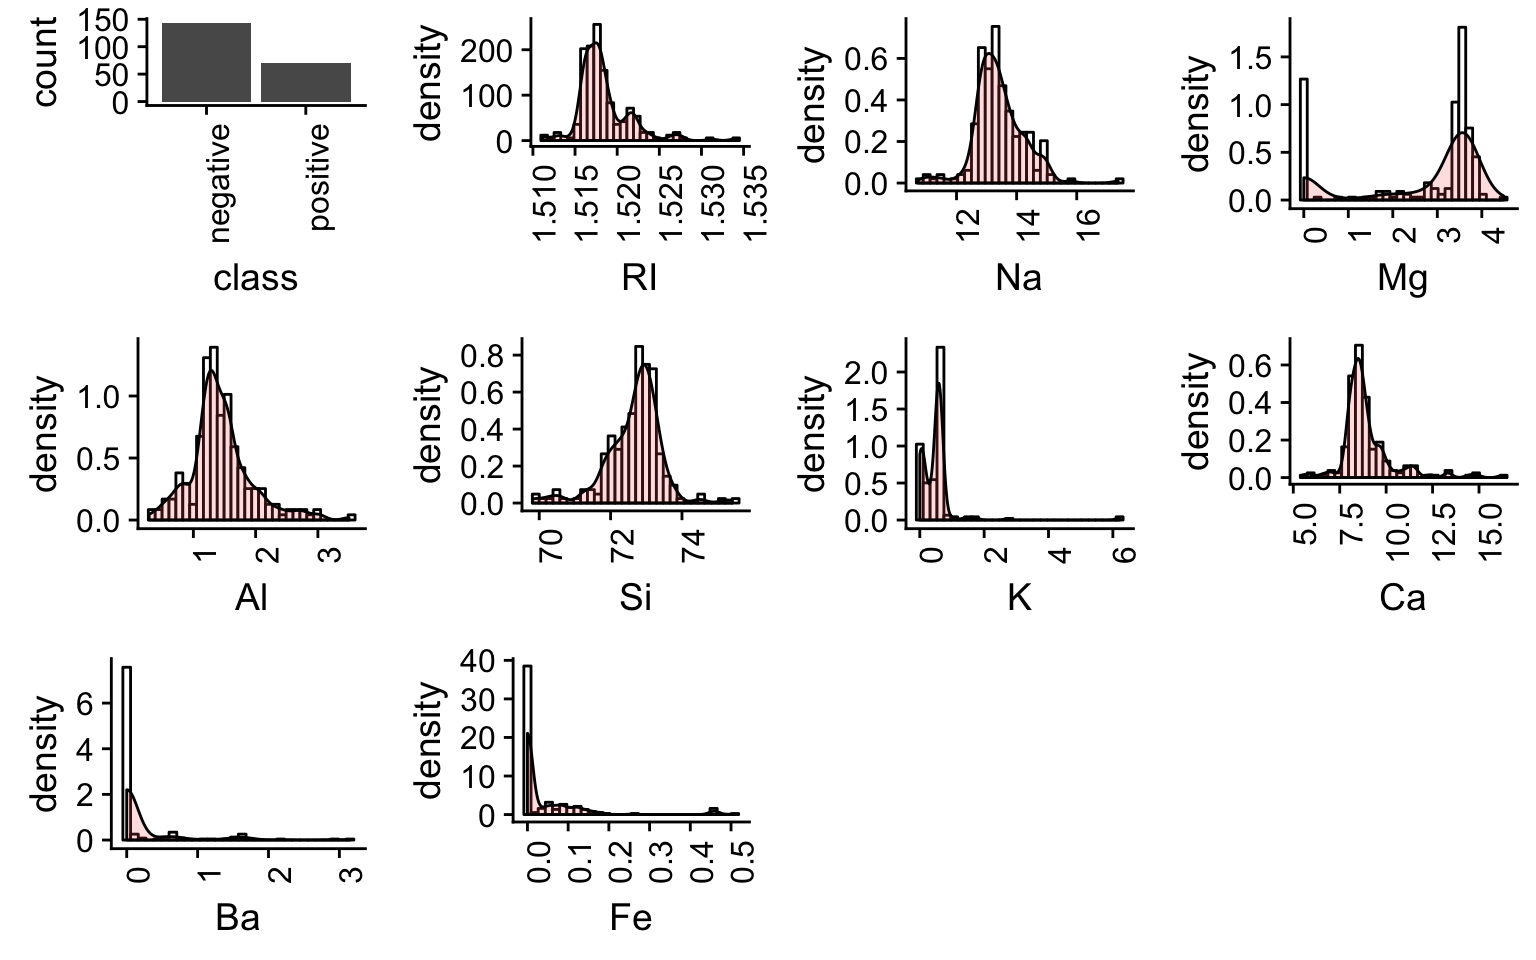
\includegraphics{Example_files/figure-latex/unnamed-chunk-24-1.pdf}

\begin{Shaded}
\begin{Highlighting}[]
\KeywordTok{ggplot}\NormalTok{() }\OperatorTok{+}
\StringTok{  }\CommentTok{# Manhattan}
\StringTok{  }\KeywordTok{geom_polygon}\NormalTok{(}\KeywordTok{aes}\NormalTok{(}\DataTypeTok{x=}\KeywordTok{c}\NormalTok{(}\OperatorTok{-}\DecValTok{3}\NormalTok{,}\DecValTok{0}\NormalTok{,}\DecValTok{3}\NormalTok{,}\DecValTok{0}\NormalTok{), }\DataTypeTok{y =} \KeywordTok{c}\NormalTok{(}\DecValTok{0}\NormalTok{,}\DecValTok{3}\NormalTok{,}\DecValTok{0}\NormalTok{,}\OperatorTok{-}\DecValTok{3}\NormalTok{), }\DataTypeTok{linetype =}\NormalTok{ b), }\DataTypeTok{fill =} \StringTok{"black"}\NormalTok{, }\DataTypeTok{color=}\NormalTok{color_manhattan, }\DataTypeTok{alpha=}\FloatTok{0.3}\NormalTok{, }\DataTypeTok{linetype =} \StringTok{"twodash"}\NormalTok{) }\OperatorTok{+}
\StringTok{  }\KeywordTok{geom_polygon}\NormalTok{(}\KeywordTok{aes}\NormalTok{(}\DataTypeTok{x=}\KeywordTok{c}\NormalTok{(}\OperatorTok{-}\DecValTok{4}\NormalTok{,}\DecValTok{0}\NormalTok{,}\DecValTok{4}\NormalTok{,}\DecValTok{0}\NormalTok{), }\DataTypeTok{y =} \KeywordTok{c}\NormalTok{(}\DecValTok{0}\NormalTok{,}\DecValTok{4}\NormalTok{,}\DecValTok{0}\NormalTok{,}\OperatorTok{-}\DecValTok{4}\NormalTok{)), }\DataTypeTok{fill =} \StringTok{"black"}\NormalTok{, }\DataTypeTok{color=}\NormalTok{color_manhattan, }\DataTypeTok{alpha=}\DecValTok{0}\NormalTok{, }\DataTypeTok{linetype =} \StringTok{"twodash"}\NormalTok{) }\OperatorTok{+}
\StringTok{  }\KeywordTok{geom_polygon}\NormalTok{(}\KeywordTok{aes}\NormalTok{(}\DataTypeTok{x=}\KeywordTok{c}\NormalTok{(}\OperatorTok{-}\NormalTok{(}\KeywordTok{sqrt}\NormalTok{(}\DecValTok{7}\NormalTok{)}\OperatorTok{+}\DecValTok{1}\NormalTok{),}\DecValTok{0}\NormalTok{,(}\KeywordTok{sqrt}\NormalTok{(}\DecValTok{7}\NormalTok{)}\OperatorTok{+}\DecValTok{1}\NormalTok{),}\DecValTok{0}\NormalTok{), }\DataTypeTok{y =} \KeywordTok{c}\NormalTok{(}\DecValTok{0}\NormalTok{,(}\KeywordTok{sqrt}\NormalTok{(}\DecValTok{7}\NormalTok{)}\OperatorTok{+}\DecValTok{1}\NormalTok{),}\DecValTok{0}\NormalTok{,}\OperatorTok{-}\NormalTok{(}\KeywordTok{sqrt}\NormalTok{(}\DecValTok{7}\NormalTok{)}\OperatorTok{+}\DecValTok{1}\NormalTok{))), }\DataTypeTok{fill =} \StringTok{"black"}\NormalTok{, }\DataTypeTok{color=}\NormalTok{color_manhattan, }\DataTypeTok{alpha=}\DecValTok{0}\NormalTok{, }\DataTypeTok{linetype =} \StringTok{"twodash"}\NormalTok{) }\OperatorTok{+}
\StringTok{ }\CommentTok{# Euclidean}
\StringTok{  }\KeywordTok{geom_circle}\NormalTok{(}\KeywordTok{aes}\NormalTok{(}\DataTypeTok{x0 =} \DecValTok{0}\NormalTok{, }\DataTypeTok{y0 =} \DecValTok{0}\NormalTok{, }\DataTypeTok{r =} \KeywordTok{sqrt}\NormalTok{(}\DecValTok{5}\NormalTok{)),  }\DataTypeTok{color=}\NormalTok{color_euclidean, }\DataTypeTok{linetype =} \StringTok{"dotted"}\NormalTok{) }\OperatorTok{+}
\StringTok{  }\KeywordTok{geom_circle}\NormalTok{(}\KeywordTok{aes}\NormalTok{(}\DataTypeTok{x0 =} \DecValTok{0}\NormalTok{, }\DataTypeTok{y0 =} \DecValTok{0}\NormalTok{, }\DataTypeTok{r =} \KeywordTok{sqrt}\NormalTok{(}\DecValTok{8}\NormalTok{)),  }\DataTypeTok{color=}\NormalTok{color_euclidean, }\DataTypeTok{linetype =} \StringTok{"dotted"}\NormalTok{) }\OperatorTok{+}
\StringTok{  }\KeywordTok{geom_circle}\NormalTok{(}\KeywordTok{aes}\NormalTok{(}\DataTypeTok{x0 =} \DecValTok{0}\NormalTok{, }\DataTypeTok{y0 =} \DecValTok{0}\NormalTok{, }\DataTypeTok{r =} \DecValTok{3}\NormalTok{),  }\DataTypeTok{color=}\NormalTok{color_euclidean, }\DataTypeTok{linetype =} \StringTok{"dotted"}\NormalTok{) }\OperatorTok{+}
\StringTok{  }\CommentTok{# Chebyshev}
\StringTok{  }\KeywordTok{geom_rect}\NormalTok{(}\KeywordTok{aes}\NormalTok{(}\DataTypeTok{xmin=}\OperatorTok{-}\DecValTok{2}\NormalTok{, }\DataTypeTok{ymin=}\OperatorTok{-}\DecValTok{2}\NormalTok{, }\DataTypeTok{xmax=}\DecValTok{2}\NormalTok{, }\DataTypeTok{ymax=}\DecValTok{2}\NormalTok{), }\DataTypeTok{fill =} \StringTok{"black"}\NormalTok{, }\DataTypeTok{color=}\NormalTok{color_chebyshev, }\DataTypeTok{alpha=}\DecValTok{0}\NormalTok{, }\DataTypeTok{linetype =} \StringTok{"longdash"}\NormalTok{) }\OperatorTok{+}
\StringTok{  }\KeywordTok{geom_rect}\NormalTok{(}\KeywordTok{aes}\NormalTok{(}\DataTypeTok{xmin=}\OperatorTok{-}\DecValTok{3}\NormalTok{, }\DataTypeTok{ymin=}\OperatorTok{-}\DecValTok{3}\NormalTok{, }\DataTypeTok{xmax=}\DecValTok{3}\NormalTok{, }\DataTypeTok{ymax=}\DecValTok{3}\NormalTok{), }\DataTypeTok{fill =} \StringTok{"black"}\NormalTok{, }\DataTypeTok{color=}\NormalTok{color_chebyshev, }\DataTypeTok{alpha=}\DecValTok{0}\NormalTok{, }\DataTypeTok{linetype =} \StringTok{"longdash"}\NormalTok{) }\OperatorTok{+}
\StringTok{  }\KeywordTok{geom_rect}\NormalTok{(}\KeywordTok{aes}\NormalTok{(}\DataTypeTok{xmin=}\OperatorTok{-}\NormalTok{(}\KeywordTok{sqrt}\NormalTok{(}\DecValTok{7}\NormalTok{)), }\DataTypeTok{ymin=}\OperatorTok{-}\NormalTok{(}\KeywordTok{sqrt}\NormalTok{(}\DecValTok{7}\NormalTok{)), }\DataTypeTok{xmax=}\NormalTok{(}\KeywordTok{sqrt}\NormalTok{(}\DecValTok{7}\NormalTok{)), }\DataTypeTok{ymax=}\NormalTok{(}\KeywordTok{sqrt}\NormalTok{(}\DecValTok{7}\NormalTok{))), }\DataTypeTok{fill =} \StringTok{"black"}\NormalTok{, }\DataTypeTok{color=}\NormalTok{color_chebyshev, }\DataTypeTok{alpha=}\DecValTok{0}\NormalTok{, }\DataTypeTok{linetype =} \StringTok{"longdash"}\NormalTok{) }\OperatorTok{+}
\StringTok{  }\CommentTok{# Plot}
\StringTok{  }\KeywordTok{geom_point}\NormalTok{(}\KeywordTok{aes}\NormalTok{(x, y, }\DataTypeTok{shape =}\NormalTok{ class, }\DataTypeTok{color =}\NormalTok{ class), }\DataTypeTok{data =}\NormalTok{ points, }\DataTypeTok{size =} \DecValTok{5}\NormalTok{) }\OperatorTok{+}
\StringTok{  }\KeywordTok{geom_text}\NormalTok{(}\KeywordTok{aes}\NormalTok{(x, y, }\DataTypeTok{label =}\NormalTok{ name), }\DataTypeTok{data =}\NormalTok{ points, }\DataTypeTok{color =} \StringTok{"white"}\NormalTok{, }\DataTypeTok{fontface =} \StringTok{"bold"}\NormalTok{, }\DataTypeTok{size =} \DecValTok{3}\NormalTok{) }\OperatorTok{+}
\StringTok{  }
\StringTok{   }\KeywordTok{scale_x_continuous}\NormalTok{(}\DataTypeTok{limits =} \KeywordTok{c}\NormalTok{(}\OperatorTok{-}\DecValTok{4}\NormalTok{, }\DecValTok{4}\NormalTok{), }\DataTypeTok{breaks =} \DecValTok{-4}\OperatorTok{:}\DecValTok{4}\NormalTok{) }\OperatorTok{+}
\StringTok{  }\KeywordTok{scale_y_continuous}\NormalTok{(}\DataTypeTok{limits =} \KeywordTok{c}\NormalTok{(}\OperatorTok{-}\DecValTok{4}\NormalTok{, }\DecValTok{4}\NormalTok{), }\DataTypeTok{breaks =} \DecValTok{-4}\OperatorTok{:}\DecValTok{4}\NormalTok{) }\OperatorTok{+}
\StringTok{  }\KeywordTok{scale_colour_manual}\NormalTok{(}\DataTypeTok{values =} \KeywordTok{c}\NormalTok{(}\StringTok{"DimGray"}\NormalTok{, }\StringTok{"Orchid"}\NormalTok{, }\StringTok{"Dark Cyan"}\NormalTok{)) }\OperatorTok{+}
\StringTok{  }\KeywordTok{coord_fixed}\NormalTok{() }\OperatorTok{+}
\StringTok{  }
\StringTok{  }\KeywordTok{theme_light}\NormalTok{() }\OperatorTok{+}
\StringTok{  }\KeywordTok{theme}\NormalTok{(}\DataTypeTok{legend.position =} \StringTok{"none"}\NormalTok{) }\OperatorTok{+}
\StringTok{  }\KeywordTok{xlab}\NormalTok{(}\StringTok{"x"}\NormalTok{) }\OperatorTok{+}
\StringTok{  }\KeywordTok{ylab}\NormalTok{(}\StringTok{"y"}\NormalTok{)}
\end{Highlighting}
\end{Shaded}

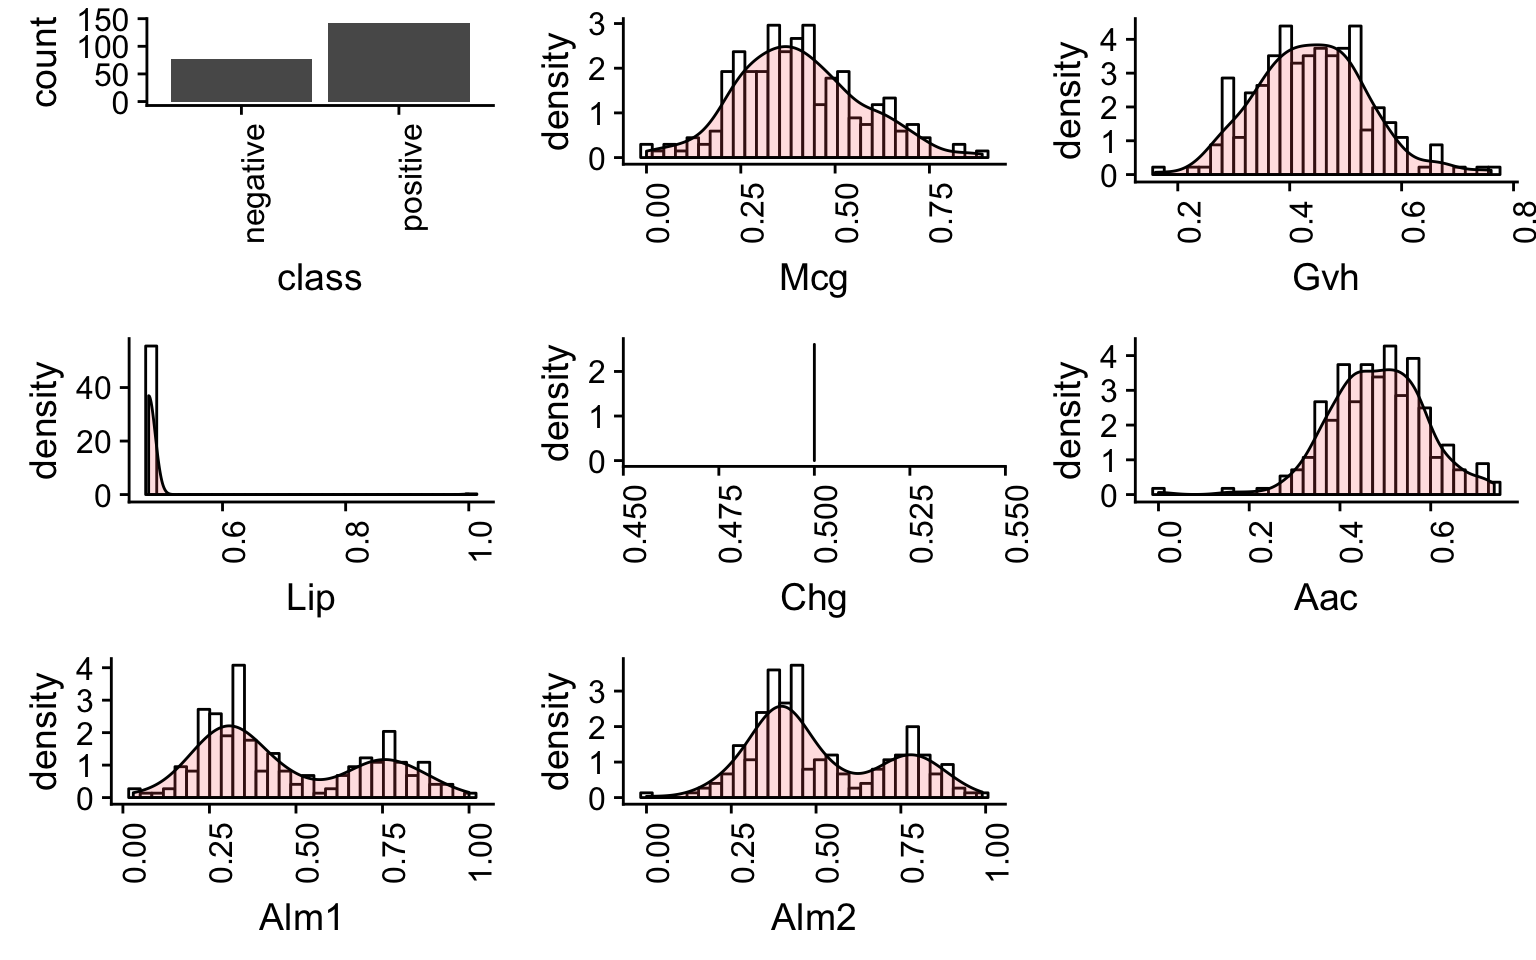
\includegraphics{Example_files/figure-latex/unnamed-chunk-25-1.pdf}

\begin{Shaded}
\begin{Highlighting}[]
\KeywordTok{ggplot}\NormalTok{() }\OperatorTok{+}
\StringTok{  }\CommentTok{# Manhattan}
\StringTok{  }\KeywordTok{geom_polygon}\NormalTok{(}\KeywordTok{aes}\NormalTok{(}\DataTypeTok{x=}\KeywordTok{c}\NormalTok{(}\OperatorTok{-}\DecValTok{3}\NormalTok{,}\DecValTok{0}\NormalTok{,}\DecValTok{3}\NormalTok{,}\DecValTok{0}\NormalTok{), }\DataTypeTok{y =} \KeywordTok{c}\NormalTok{(}\DecValTok{0}\NormalTok{,}\DecValTok{3}\NormalTok{,}\DecValTok{0}\NormalTok{,}\OperatorTok{-}\DecValTok{3}\NormalTok{), }\DataTypeTok{linetype =}\NormalTok{ b), }\DataTypeTok{fill =} \StringTok{"black"}\NormalTok{, }\DataTypeTok{color=}\NormalTok{color_manhattan, }\DataTypeTok{alpha=}\DecValTok{0}\NormalTok{, }\DataTypeTok{linetype =} \StringTok{"twodash"}\NormalTok{) }\OperatorTok{+}
\StringTok{  }\KeywordTok{geom_polygon}\NormalTok{(}\KeywordTok{aes}\NormalTok{(}\DataTypeTok{x=}\KeywordTok{c}\NormalTok{(}\OperatorTok{-}\DecValTok{4}\NormalTok{,}\DecValTok{0}\NormalTok{,}\DecValTok{4}\NormalTok{,}\DecValTok{0}\NormalTok{), }\DataTypeTok{y =} \KeywordTok{c}\NormalTok{(}\DecValTok{0}\NormalTok{,}\DecValTok{4}\NormalTok{,}\DecValTok{0}\NormalTok{,}\OperatorTok{-}\DecValTok{4}\NormalTok{)), }\DataTypeTok{fill =} \StringTok{"black"}\NormalTok{, }\DataTypeTok{color=}\NormalTok{color_manhattan, }\DataTypeTok{alpha=}\DecValTok{0}\NormalTok{, }\DataTypeTok{linetype =} \StringTok{"twodash"}\NormalTok{) }\OperatorTok{+}
\StringTok{  }\KeywordTok{geom_polygon}\NormalTok{(}\KeywordTok{aes}\NormalTok{(}\DataTypeTok{x=}\KeywordTok{c}\NormalTok{(}\OperatorTok{-}\NormalTok{(}\KeywordTok{sqrt}\NormalTok{(}\DecValTok{7}\NormalTok{)}\OperatorTok{+}\DecValTok{1}\NormalTok{),}\DecValTok{0}\NormalTok{,(}\KeywordTok{sqrt}\NormalTok{(}\DecValTok{7}\NormalTok{)}\OperatorTok{+}\DecValTok{1}\NormalTok{),}\DecValTok{0}\NormalTok{), }\DataTypeTok{y =} \KeywordTok{c}\NormalTok{(}\DecValTok{0}\NormalTok{,(}\KeywordTok{sqrt}\NormalTok{(}\DecValTok{7}\NormalTok{)}\OperatorTok{+}\DecValTok{1}\NormalTok{),}\DecValTok{0}\NormalTok{,}\OperatorTok{-}\NormalTok{(}\KeywordTok{sqrt}\NormalTok{(}\DecValTok{7}\NormalTok{)}\OperatorTok{+}\DecValTok{1}\NormalTok{))), }\DataTypeTok{fill =} \StringTok{"black"}\NormalTok{, }\DataTypeTok{color=}\NormalTok{color_manhattan, }\DataTypeTok{alpha=}\DecValTok{0}\NormalTok{, }\DataTypeTok{linetype =} \StringTok{"twodash"}\NormalTok{) }\OperatorTok{+}
\StringTok{ }\CommentTok{# Euclidean}
\StringTok{  }\KeywordTok{geom_circle}\NormalTok{(}\KeywordTok{aes}\NormalTok{(}\DataTypeTok{x0 =} \DecValTok{0}\NormalTok{, }\DataTypeTok{y0 =} \DecValTok{0}\NormalTok{, }\DataTypeTok{r =} \KeywordTok{sqrt}\NormalTok{(}\DecValTok{5}\NormalTok{)),  }\DataTypeTok{color=}\NormalTok{color_euclidean, }\DataTypeTok{linetype =} \StringTok{"dotted"}\NormalTok{) }\OperatorTok{+}
\StringTok{  }\KeywordTok{geom_circle}\NormalTok{(}\KeywordTok{aes}\NormalTok{(}\DataTypeTok{x0 =} \DecValTok{0}\NormalTok{, }\DataTypeTok{y0 =} \DecValTok{0}\NormalTok{, }\DataTypeTok{r =} \KeywordTok{sqrt}\NormalTok{(}\DecValTok{8}\NormalTok{)),  }\DataTypeTok{color=}\NormalTok{color_euclidean, }\DataTypeTok{linetype =} \StringTok{"dotted"}\NormalTok{, }\DataTypeTok{fill =} \StringTok{"black"}\NormalTok{, }\DataTypeTok{alpha=}\FloatTok{0.3}\NormalTok{) }\OperatorTok{+}
\StringTok{  }\KeywordTok{geom_circle}\NormalTok{(}\KeywordTok{aes}\NormalTok{(}\DataTypeTok{x0 =} \DecValTok{0}\NormalTok{, }\DataTypeTok{y0 =} \DecValTok{0}\NormalTok{, }\DataTypeTok{r =} \DecValTok{3}\NormalTok{),  }\DataTypeTok{color=}\NormalTok{color_euclidean, }\DataTypeTok{linetype =} \StringTok{"dotted"}\NormalTok{) }\OperatorTok{+}
\StringTok{  }\CommentTok{# Chebyshev}
\StringTok{  }\KeywordTok{geom_rect}\NormalTok{(}\KeywordTok{aes}\NormalTok{(}\DataTypeTok{xmin=}\OperatorTok{-}\DecValTok{2}\NormalTok{, }\DataTypeTok{ymin=}\OperatorTok{-}\DecValTok{2}\NormalTok{, }\DataTypeTok{xmax=}\DecValTok{2}\NormalTok{, }\DataTypeTok{ymax=}\DecValTok{2}\NormalTok{), }\DataTypeTok{fill =} \StringTok{"black"}\NormalTok{, }\DataTypeTok{color=}\NormalTok{color_chebyshev, }\DataTypeTok{alpha=}\DecValTok{0}\NormalTok{, }\DataTypeTok{linetype =} \StringTok{"longdash"}\NormalTok{) }\OperatorTok{+}
\StringTok{  }\KeywordTok{geom_rect}\NormalTok{(}\KeywordTok{aes}\NormalTok{(}\DataTypeTok{xmin=}\OperatorTok{-}\DecValTok{3}\NormalTok{, }\DataTypeTok{ymin=}\OperatorTok{-}\DecValTok{3}\NormalTok{, }\DataTypeTok{xmax=}\DecValTok{3}\NormalTok{, }\DataTypeTok{ymax=}\DecValTok{3}\NormalTok{), }\DataTypeTok{fill =} \StringTok{"black"}\NormalTok{, }\DataTypeTok{color=}\NormalTok{color_chebyshev, }\DataTypeTok{alpha=}\DecValTok{0}\NormalTok{, }\DataTypeTok{linetype =} \StringTok{"longdash"}\NormalTok{) }\OperatorTok{+}
\StringTok{  }\KeywordTok{geom_rect}\NormalTok{(}\KeywordTok{aes}\NormalTok{(}\DataTypeTok{xmin=}\OperatorTok{-}\NormalTok{(}\KeywordTok{sqrt}\NormalTok{(}\DecValTok{7}\NormalTok{)), }\DataTypeTok{ymin=}\OperatorTok{-}\NormalTok{(}\KeywordTok{sqrt}\NormalTok{(}\DecValTok{7}\NormalTok{)), }\DataTypeTok{xmax=}\NormalTok{(}\KeywordTok{sqrt}\NormalTok{(}\DecValTok{7}\NormalTok{)), }\DataTypeTok{ymax=}\NormalTok{(}\KeywordTok{sqrt}\NormalTok{(}\DecValTok{7}\NormalTok{))), }\DataTypeTok{fill =} \StringTok{"black"}\NormalTok{, }\DataTypeTok{color=}\NormalTok{color_chebyshev, }\DataTypeTok{alpha=}\DecValTok{0}\NormalTok{, }\DataTypeTok{linetype =} \StringTok{"longdash"}\NormalTok{) }\OperatorTok{+}
\StringTok{  }\CommentTok{# Plot}
\StringTok{  }\KeywordTok{geom_point}\NormalTok{(}\KeywordTok{aes}\NormalTok{(x, y, }\DataTypeTok{shape =}\NormalTok{ class, }\DataTypeTok{color =}\NormalTok{ class), }\DataTypeTok{data =}\NormalTok{ points, }\DataTypeTok{size =} \DecValTok{5}\NormalTok{) }\OperatorTok{+}
\StringTok{  }\KeywordTok{geom_text}\NormalTok{(}\KeywordTok{aes}\NormalTok{(x, y, }\DataTypeTok{label =}\NormalTok{ name), }\DataTypeTok{data =}\NormalTok{ points, }\DataTypeTok{color =} \StringTok{"white"}\NormalTok{, }\DataTypeTok{fontface =} \StringTok{"bold"}\NormalTok{, }\DataTypeTok{size =} \DecValTok{3}\NormalTok{) }\OperatorTok{+}
\StringTok{  }
\StringTok{   }\KeywordTok{scale_x_continuous}\NormalTok{(}\DataTypeTok{limits =} \KeywordTok{c}\NormalTok{(}\OperatorTok{-}\DecValTok{4}\NormalTok{, }\DecValTok{4}\NormalTok{), }\DataTypeTok{breaks =} \DecValTok{-4}\OperatorTok{:}\DecValTok{4}\NormalTok{) }\OperatorTok{+}
\StringTok{  }\KeywordTok{scale_y_continuous}\NormalTok{(}\DataTypeTok{limits =} \KeywordTok{c}\NormalTok{(}\OperatorTok{-}\DecValTok{4}\NormalTok{, }\DecValTok{4}\NormalTok{), }\DataTypeTok{breaks =} \DecValTok{-4}\OperatorTok{:}\DecValTok{4}\NormalTok{) }\OperatorTok{+}
\StringTok{  }\KeywordTok{scale_colour_manual}\NormalTok{(}\DataTypeTok{values =} \KeywordTok{c}\NormalTok{(}\StringTok{"DimGray"}\NormalTok{, }\StringTok{"Orchid"}\NormalTok{, }\StringTok{"Dark Cyan"}\NormalTok{)) }\OperatorTok{+}
\StringTok{  }\KeywordTok{coord_fixed}\NormalTok{() }\OperatorTok{+}
\StringTok{  }
\StringTok{  }\KeywordTok{theme_light}\NormalTok{() }\OperatorTok{+}
\StringTok{  }\KeywordTok{theme}\NormalTok{(}\DataTypeTok{legend.position =} \StringTok{"none"}\NormalTok{) }\OperatorTok{+}
\StringTok{  }\KeywordTok{xlab}\NormalTok{(}\StringTok{"x"}\NormalTok{) }\OperatorTok{+}
\StringTok{  }\KeywordTok{ylab}\NormalTok{(}\StringTok{"y"}\NormalTok{)}
\end{Highlighting}
\end{Shaded}

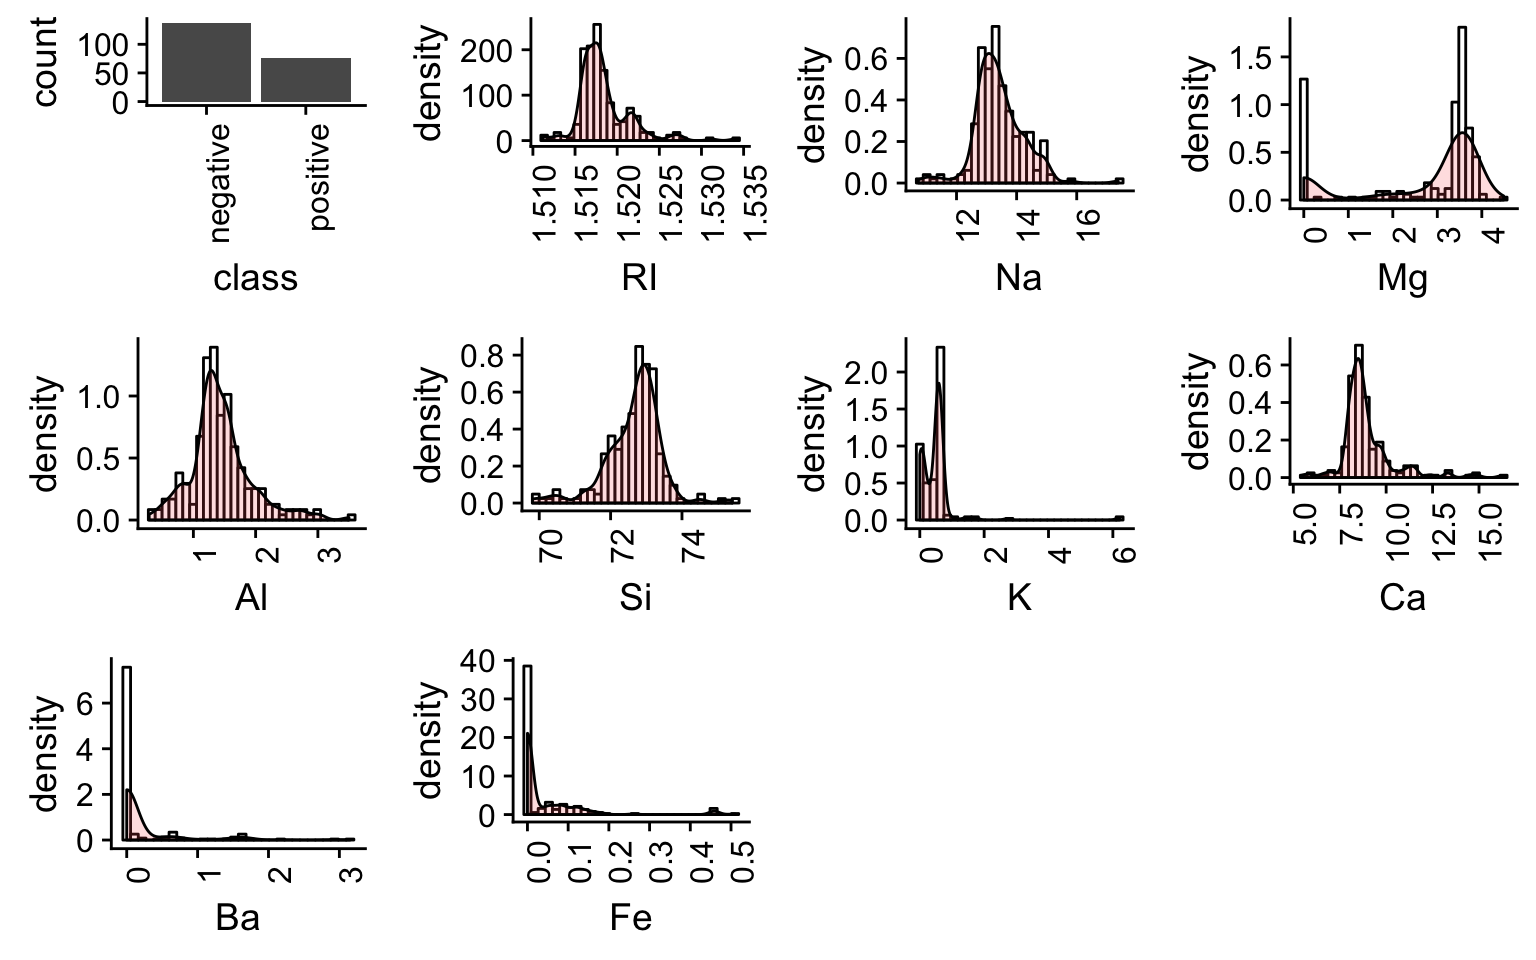
\includegraphics{Example_files/figure-latex/unnamed-chunk-26-1.pdf}

\begin{Shaded}
\begin{Highlighting}[]
\KeywordTok{ggplot}\NormalTok{() }\OperatorTok{+}
\StringTok{  }\CommentTok{# Manhattan}
\StringTok{  }\KeywordTok{geom_polygon}\NormalTok{(}\KeywordTok{aes}\NormalTok{(}\DataTypeTok{x=}\KeywordTok{c}\NormalTok{(}\OperatorTok{-}\DecValTok{3}\NormalTok{,}\DecValTok{0}\NormalTok{,}\DecValTok{3}\NormalTok{,}\DecValTok{0}\NormalTok{), }\DataTypeTok{y =} \KeywordTok{c}\NormalTok{(}\DecValTok{0}\NormalTok{,}\DecValTok{3}\NormalTok{,}\DecValTok{0}\NormalTok{,}\OperatorTok{-}\DecValTok{3}\NormalTok{), }\DataTypeTok{linetype =}\NormalTok{ b), }\DataTypeTok{fill =} \StringTok{"black"}\NormalTok{, }\DataTypeTok{color=}\NormalTok{color_manhattan, }\DataTypeTok{alpha=}\DecValTok{0}\NormalTok{, }\DataTypeTok{linetype =} \StringTok{"twodash"}\NormalTok{) }\OperatorTok{+}
\StringTok{  }\KeywordTok{geom_polygon}\NormalTok{(}\KeywordTok{aes}\NormalTok{(}\DataTypeTok{x=}\KeywordTok{c}\NormalTok{(}\OperatorTok{-}\DecValTok{4}\NormalTok{,}\DecValTok{0}\NormalTok{,}\DecValTok{4}\NormalTok{,}\DecValTok{0}\NormalTok{), }\DataTypeTok{y =} \KeywordTok{c}\NormalTok{(}\DecValTok{0}\NormalTok{,}\DecValTok{4}\NormalTok{,}\DecValTok{0}\NormalTok{,}\OperatorTok{-}\DecValTok{4}\NormalTok{)), }\DataTypeTok{fill =} \StringTok{"black"}\NormalTok{, }\DataTypeTok{color=}\NormalTok{color_manhattan, }\DataTypeTok{alpha=}\DecValTok{0}\NormalTok{, }\DataTypeTok{linetype =} \StringTok{"twodash"}\NormalTok{) }\OperatorTok{+}
\StringTok{  }\KeywordTok{geom_polygon}\NormalTok{(}\KeywordTok{aes}\NormalTok{(}\DataTypeTok{x=}\KeywordTok{c}\NormalTok{(}\OperatorTok{-}\NormalTok{(}\KeywordTok{sqrt}\NormalTok{(}\DecValTok{7}\NormalTok{)}\OperatorTok{+}\DecValTok{1}\NormalTok{),}\DecValTok{0}\NormalTok{,(}\KeywordTok{sqrt}\NormalTok{(}\DecValTok{7}\NormalTok{)}\OperatorTok{+}\DecValTok{1}\NormalTok{),}\DecValTok{0}\NormalTok{), }\DataTypeTok{y =} \KeywordTok{c}\NormalTok{(}\DecValTok{0}\NormalTok{,(}\KeywordTok{sqrt}\NormalTok{(}\DecValTok{7}\NormalTok{)}\OperatorTok{+}\DecValTok{1}\NormalTok{),}\DecValTok{0}\NormalTok{,}\OperatorTok{-}\NormalTok{(}\KeywordTok{sqrt}\NormalTok{(}\DecValTok{7}\NormalTok{)}\OperatorTok{+}\DecValTok{1}\NormalTok{))), }\DataTypeTok{fill =} \StringTok{"black"}\NormalTok{, }\DataTypeTok{color=}\NormalTok{color_manhattan, }\DataTypeTok{alpha=}\DecValTok{0}\NormalTok{, }\DataTypeTok{linetype =} \StringTok{"twodash"}\NormalTok{) }\OperatorTok{+}
\StringTok{ }\CommentTok{# Euclidean}
\StringTok{  }\KeywordTok{geom_circle}\NormalTok{(}\KeywordTok{aes}\NormalTok{(}\DataTypeTok{x0 =} \DecValTok{0}\NormalTok{, }\DataTypeTok{y0 =} \DecValTok{0}\NormalTok{, }\DataTypeTok{r =} \KeywordTok{sqrt}\NormalTok{(}\DecValTok{5}\NormalTok{)),  }\DataTypeTok{color=}\NormalTok{color_euclidean, }\DataTypeTok{linetype =} \StringTok{"dotted"}\NormalTok{) }\OperatorTok{+}
\StringTok{  }\KeywordTok{geom_circle}\NormalTok{(}\KeywordTok{aes}\NormalTok{(}\DataTypeTok{x0 =} \DecValTok{0}\NormalTok{, }\DataTypeTok{y0 =} \DecValTok{0}\NormalTok{, }\DataTypeTok{r =} \KeywordTok{sqrt}\NormalTok{(}\DecValTok{8}\NormalTok{)),  }\DataTypeTok{color=}\NormalTok{color_euclidean, }\DataTypeTok{linetype =} \StringTok{"dotted"}\NormalTok{, }\DataTypeTok{fill =} \StringTok{"black"}\NormalTok{, }\DataTypeTok{alpha=}\DecValTok{0}\NormalTok{) }\OperatorTok{+}
\StringTok{  }\KeywordTok{geom_circle}\NormalTok{(}\KeywordTok{aes}\NormalTok{(}\DataTypeTok{x0 =} \DecValTok{0}\NormalTok{, }\DataTypeTok{y0 =} \DecValTok{0}\NormalTok{, }\DataTypeTok{r =} \DecValTok{3}\NormalTok{),  }\DataTypeTok{color=}\NormalTok{color_euclidean, }\DataTypeTok{linetype =} \StringTok{"dotted"}\NormalTok{) }\OperatorTok{+}
\StringTok{  }\CommentTok{# Chebyshev}
\StringTok{  }\KeywordTok{geom_rect}\NormalTok{(}\KeywordTok{aes}\NormalTok{(}\DataTypeTok{xmin=}\OperatorTok{-}\DecValTok{2}\NormalTok{, }\DataTypeTok{ymin=}\OperatorTok{-}\DecValTok{2}\NormalTok{, }\DataTypeTok{xmax=}\DecValTok{2}\NormalTok{, }\DataTypeTok{ymax=}\DecValTok{2}\NormalTok{), }\DataTypeTok{fill =} \StringTok{"black"}\NormalTok{, }\DataTypeTok{color=}\NormalTok{color_chebyshev, }\DataTypeTok{alpha=}\FloatTok{0.3}\NormalTok{, }\DataTypeTok{linetype =} \StringTok{"longdash"}\NormalTok{) }\OperatorTok{+}
\StringTok{  }\KeywordTok{geom_rect}\NormalTok{(}\KeywordTok{aes}\NormalTok{(}\DataTypeTok{xmin=}\OperatorTok{-}\DecValTok{3}\NormalTok{, }\DataTypeTok{ymin=}\OperatorTok{-}\DecValTok{3}\NormalTok{, }\DataTypeTok{xmax=}\DecValTok{3}\NormalTok{, }\DataTypeTok{ymax=}\DecValTok{3}\NormalTok{), }\DataTypeTok{fill =} \StringTok{"black"}\NormalTok{, }\DataTypeTok{color=}\NormalTok{color_chebyshev, }\DataTypeTok{alpha=}\DecValTok{0}\NormalTok{, }\DataTypeTok{linetype =} \StringTok{"longdash"}\NormalTok{) }\OperatorTok{+}
\StringTok{  }\KeywordTok{geom_rect}\NormalTok{(}\KeywordTok{aes}\NormalTok{(}\DataTypeTok{xmin=}\OperatorTok{-}\NormalTok{(}\KeywordTok{sqrt}\NormalTok{(}\DecValTok{7}\NormalTok{)), }\DataTypeTok{ymin=}\OperatorTok{-}\NormalTok{(}\KeywordTok{sqrt}\NormalTok{(}\DecValTok{7}\NormalTok{)), }\DataTypeTok{xmax=}\NormalTok{(}\KeywordTok{sqrt}\NormalTok{(}\DecValTok{7}\NormalTok{)), }\DataTypeTok{ymax=}\NormalTok{(}\KeywordTok{sqrt}\NormalTok{(}\DecValTok{7}\NormalTok{))), }\DataTypeTok{fill =} \StringTok{"black"}\NormalTok{, }\DataTypeTok{color=}\NormalTok{color_chebyshev, }\DataTypeTok{alpha=}\DecValTok{0}\NormalTok{, }\DataTypeTok{linetype =} \StringTok{"longdash"}\NormalTok{) }\OperatorTok{+}
\StringTok{  }\CommentTok{# Plot}
\StringTok{  }\KeywordTok{geom_point}\NormalTok{(}\KeywordTok{aes}\NormalTok{(x, y, }\DataTypeTok{shape =}\NormalTok{ class, }\DataTypeTok{color =}\NormalTok{ class), }\DataTypeTok{data =}\NormalTok{ points, }\DataTypeTok{size =} \DecValTok{5}\NormalTok{) }\OperatorTok{+}
\StringTok{  }\KeywordTok{geom_text}\NormalTok{(}\KeywordTok{aes}\NormalTok{(x, y, }\DataTypeTok{label =}\NormalTok{ name), }\DataTypeTok{data =}\NormalTok{ points, }\DataTypeTok{color =} \StringTok{"white"}\NormalTok{, }\DataTypeTok{fontface =} \StringTok{"bold"}\NormalTok{, }\DataTypeTok{size =} \DecValTok{3}\NormalTok{) }\OperatorTok{+}
\StringTok{  }
\StringTok{   }\KeywordTok{scale_x_continuous}\NormalTok{(}\DataTypeTok{limits =} \KeywordTok{c}\NormalTok{(}\OperatorTok{-}\DecValTok{4}\NormalTok{, }\DecValTok{4}\NormalTok{), }\DataTypeTok{breaks =} \DecValTok{-4}\OperatorTok{:}\DecValTok{4}\NormalTok{) }\OperatorTok{+}
\StringTok{  }\KeywordTok{scale_y_continuous}\NormalTok{(}\DataTypeTok{limits =} \KeywordTok{c}\NormalTok{(}\OperatorTok{-}\DecValTok{4}\NormalTok{, }\DecValTok{4}\NormalTok{), }\DataTypeTok{breaks =} \DecValTok{-4}\OperatorTok{:}\DecValTok{4}\NormalTok{) }\OperatorTok{+}
\StringTok{  }\KeywordTok{scale_colour_manual}\NormalTok{(}\DataTypeTok{values =} \KeywordTok{c}\NormalTok{(}\StringTok{"DimGray"}\NormalTok{, }\StringTok{"Orchid"}\NormalTok{, }\StringTok{"Dark Cyan"}\NormalTok{)) }\OperatorTok{+}
\StringTok{  }\KeywordTok{coord_fixed}\NormalTok{() }\OperatorTok{+}
\StringTok{  }
\StringTok{  }\KeywordTok{theme_light}\NormalTok{() }\OperatorTok{+}
\StringTok{  }\KeywordTok{theme}\NormalTok{(}\DataTypeTok{legend.position =} \StringTok{"none"}\NormalTok{) }\OperatorTok{+}
\StringTok{  }\KeywordTok{xlab}\NormalTok{(}\StringTok{"x"}\NormalTok{) }\OperatorTok{+}
\StringTok{  }\KeywordTok{ylab}\NormalTok{(}\StringTok{"y"}\NormalTok{)}
\end{Highlighting}
\end{Shaded}

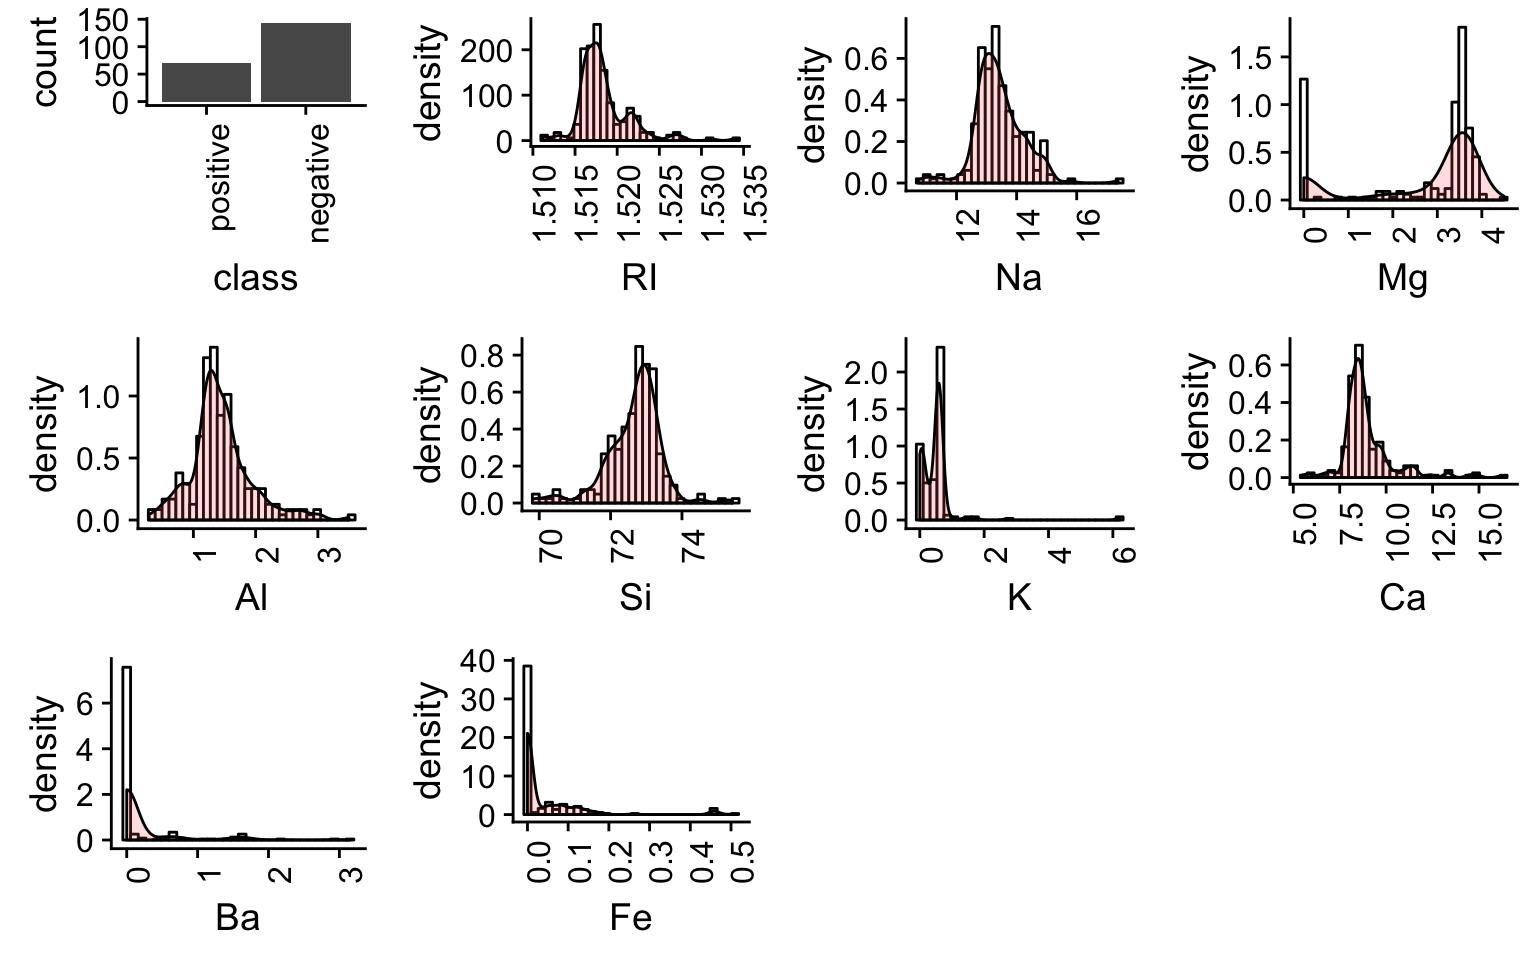
\includegraphics{Example_files/figure-latex/unnamed-chunk-27-1.pdf}


\end{document}
